\part{Preliminaries}
    \chapter{Set Theory}
        This chapter will cover the necessary prerequisites before we dive into
        the various areas of mathematical analysis. This will include a short
        course on set theory and logic. We will develop set theory from the
        axioms known as Zermelo-Fraenkel Set Theory, together with the Axiom of
        Choice, commonly abbreviated as ZFC.
        \section{Basic Notions}
    \begin{ldefinition}{Sets}{Sets}
        A \gls{set} is a collection of objects, called elements, none of which
        is the set itself. Given a set $A$ and an element $x$, we denote that
        $x$ is contained in $A$ by writing $x\in{A}$. If $x$ is not an
        element of $A$, we write $x\notin{A}$.
    \end{ldefinition}
    The notion of a \textrm{set} is often left undefined, and we haven't
    defined it very well here, either. The terms \textit{collection} and
    \textit{object} have not been defined, and thus this definition is
    somewhat meaningless. Intuitively, a set is a bunch of things that we can
    discuss, either by the properties these things have, or by listing them
    out.
    \begin{lexample}{Basic Sets}{Example_of_Basic_Sets}
        When possible it is convenient to simply list out the elements of a
        set. The standard notation is to enclose the elements in braces,
        separated by commas.
        \begin{equation}
            A=\{\,1,\,2,\,3\,\}
        \end{equation}
        Here, $A$ is a set and it is entirely determined by the elements 1, 2,
        and 3. Sets need not only be concerned with numbers, and we can allow
        for abstract objects.
        \par
        \begin{subequations}
            \begin{minipage}[b]{0.49\textwidth}
                \centering
                \begin{equation}
                    B=\{\,a,\,b,\,c\,\}
                \end{equation}
            \end{minipage}
            \hfill
            \begin{minipage}[b]{0.49\textwidth}
                \centering
                \begin{equation}
                    C=\{\,\textrm{Boston, New York}\,\}
                \end{equation}
            \end{minipage}
        \end{subequations}
        \par\vspace{2.5ex}
        Both of these are valid sets.
    \end{lexample}
    \begin{lexample}{}{Sets_with_Ellipses}
        The examples described in Ex.~\ref{ex:Example_of_Basic_Sets} are all
        finite and contain a small number of elements. For larger sets we use
        ellipses to indicate some pattern. For example:
        \par
        \begin{subequations}
            \begin{minipage}[b]{0.49\textwidth}
                \centering
                \begin{align}
                    \mathbb{Z}_{3}&=\{\,1,\,2,\,3\,\}\\
                    \mathbb{Z}_{4}&=\{\,1,\,2,\,3,\,4\,\}
                \end{align}
            \end{minipage}
            \hfill
            \begin{minipage}[b]{0.49\textwidth}
                \centering
                \begin{align}
                    \mathbb{Z}_{6}  &=\{\,1,\,2,\,\dots,\,5,\,6\,\}\\
                    \mathbb{Z}_{108}&=\{\,1,\,2,\,\dots,\,107,\,108\,\}
                \end{align}
            \end{minipage}
        \end{subequations}
        \par\vspace{2.5ex}
        For infinite sets it is best to use what is known as
        \textit{Set-Builder} notation, but when a pattern is clear enough
        ellipses can suffice. The set of natural numbers and the set of
        integers are often described this way:
        \begin{subequations}
            \begin{align}
                \label{eqn:Natural_Numbers_Ellipses}%
                \mathbb{N}&=\{\,1,\,2,\,3,\,\dots\,\}\\
                \label{eqn:Integers_Ellipses}%
                \mathbb{Z}&=\{\,\dots,\,\minus{3},\,\minus{2},\,\minus{1},\,
                                0,\,1,\,2,\,3,\,\dots\,\}
            \end{align}
        \end{subequations}
        Rigorous definitions for both of these sets will be given after we've
        developed set theory more thoroughly.
    \end{lexample}
    The requirement that a set cannot contain itself is to avoid various
    paradoxes, such as the one discovered by Bertrand Russell in 1901. To
    avoid such problems, Ernst Zermello proposed a collection of
    \textit{axioms} in 1908. Subtle problems were pointed out by Abraham
    Fraenkel in 1921, and eventually the system known as Zermelo-Fraenkel
    Set Theory came to be. The condition that a set cannot contain itself can
    be restated as the \textit{Axiom of Regularity}. It is phrased as follows:
    \begin{axiom}[Axiom of Regularity]
        \label{ax:Axiom_of_Regularity}%
        If $A$ is a non-empty set, then there is a set $B\in{A}$
        such that that $A$ and $B$ are disjoint.
    \end{axiom}
    We've yet to discuss what empty and non-empty means, nor have we discussed
    the definition of disjoint. Intuitively, non-empty means the set has
    \textit{something} contained in it, and disjoint sets are sets with
    nothing in common. That is, none of their elements are the same. The axiom
    of regularity implies that, given a set $A$, it is impossible for $A$
    to be an element of $A$.
    \begin{axiom}[Axiom of the Empty Set]
        \label{ax:Axiom_of_the_Empty_Set}%
        There exists a set $\emptyset$ such that, if $x$ is an element,
        then $x\notin\emptyset$.
    \end{axiom}
    This axiom is used to define and justify the existence of the empty set.
    \begin{ldefinition}{The Empty Set}{Empty_Set}
        The \gls{empty set} is the set $\emptyset$ such that,
        for all $x$, it is true that $x\notin\emptyset$.
    \end{ldefinition}
    The empty set contains no elements and we occasionally write
    $\emptyset=\{\}$. It is unique. Note that the empty set is different from
    the set $\{\emptyset\}$. Indeed, this would violate our requirement that
    sets do not contain themselves. The empty set contains no elements,
    whereas $\{\emptyset\}$ contains one element (It contains the empty set).
    \subsection{Subsets}
        A set is determined entirely by it's elements. Thus repetition of
        elements cannot be accounted for, and the sets $\{a,\,b\}$ and
        $\{a,\,a,\,b\}$ must be considered the same, since they have exactly
        the same elements. Similarly, $\{a,\,b\}$ and $\{b,\,a\}$ are the
        same. To distinguish between such things requires a notion of order.
        This is achieved by introducing the notions of \textit{ordered pairs}
        and \textit{functions}. To rigorously show that the three
        aforementioned sets are indeed the same will require a definition of
        equality.
        \begin{ldefinition}{Subsets}{Subsets}
            A \gls{subset} of a set $B$ is a set $A$, denoted $A\subseteq{B}$,
            such that for all $x\in{A}$, it is true that $x\in{B}$. We write
            $A\nsubseteq{B}$ to denote that $A$ is not a subset of $B$.
        \end{ldefinition}
        We can often picture sets and subsets as blobs in the plane
        (Fig.~\ref{fig:Subset_Blobs}). In this figure, the blob $A$ is
        entirely contained within the blob $B$, and thus $A$ is a subset of
        $B$. The definition of subset allows us to rigorously define the
        notion of equality.
        \begin{figure}[H]
            \centering
            %--------------------------------Dependencies----------------------------------%
%   tikz                                                                       %
%-------------------------------Main Document----------------------------------%
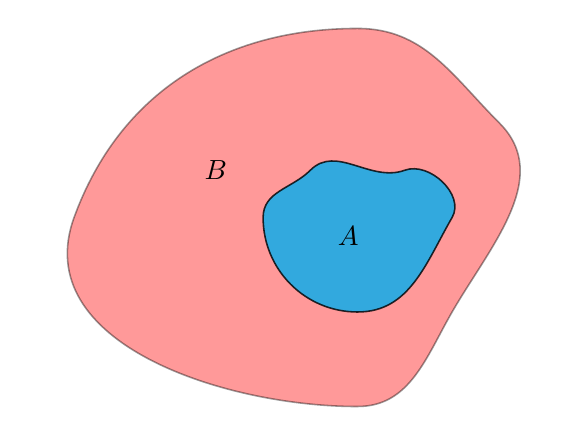
\begin{tikzpicture}[line width=0.2mm, scale=1.2]

    % Coordinates for the bigger blob.
    \coordinate (P1) at ( 0.0, -2.0);
    \coordinate (P2) at ( 1.0, -1.0);
    \coordinate (P3) at ( 1.5,  1.0);
    \coordinate (P4) at ( 0.0,  2.0);
    \coordinate (P5) at (-3.0,  0.0);

    % Coordinates for the inner blob.
    \coordinate (Q1) at ( 0.0, -1.0);
    \coordinate (Q2) at ( 1.0,  0.0);
    \coordinate (Q3) at ( 0.5,  0.5);
    \coordinate (Q4) at (-0.5,  0.5);
    \coordinate (Q5) at (-1.0,  0.0);

    % Coordindates to label things.
    \coordinate (A) at (-0.1, -0.2);
    \coordinate (B) at (-1.5,  0.5);

    % Draw the bigger blob.
    \draw[fill=red, opacity=0.4] (P1) to [out=0,    in=-120] (P2)
                                      to [out=60,   in=-45]  (P3)
                                      to [out=135,  in=0]    (P4)
                                      to [out=-180, in=70]   (P5)
                                      to [out=-110, in=-180] cycle;

    % Draw the inner blob.
    \draw[fill=cyan, opacity=0.8] (Q1) to [out=0,    in=-120]  (Q2)
                                       to [out=60,   in=20]    (Q3)
                                       to [out=-160, in=45]    (Q4)
                                       to [out=-135, in=90]    (Q5)
                                       to [out=-90,  in=180]   cycle;

    % Labels for the two blobs.
    \node at (A) {$A$};
    \node at (B) {$B$};
\end{tikzpicture}

            \caption[Visual for Subsets]
                    {Sets can be Visualized as Blobsin the Plane.}
            \label{fig:Subset_Blobs}
        \end{figure}
        \begin{lexample}{Subsets}{Basic_Subsets}
            If we let $A$ and $B$ be the sets defined by:
            \par
            \begin{subequations}
                \begin{minipage}[b]{0.49\textwidth}
                    \centering
                    \begin{equation}
                        A=\{\,1,\,2,\,3\,\}
                    \end{equation}
                \end{minipage}
                \hfill
                \begin{minipage}[b]{0.49\textwidth}
                    \centering
                    \begin{equation}
                        B=\{\,1,\,2,\,3,\,4,\,5\,\}
                    \end{equation}
                \end{minipage}
            \end{subequations}
            \par\vspace{2.5ex}
            Then we see that $A$ is a subset of $B$ since every element of
            $A$ is also an element of $B$. To express this, we write
            $A\subseteq{B}$. However, $B$ is not a subset of $A$ since the
            element 4 is contained in $B$ but it is not contained in $A$.
            Thus we may write $B\nsubseteq{A}$, indicating that $B$ is not a
            subset of $A$. Furthermore, if we define:
            \begin{equation}
                C=\{\,4,\,5,\,6,\,7,\,8\,\}
            \end{equation}
            Then we see that neither $B$ is a subset of $C$, nor is $C$ a
            subset of $B$. That is, $B\nsubseteq{C}$ and $C\nsubseteq{B}$.
            This is because $B$ has elements that aren't in $C$, and
            $C$ has elements that aren't in $B$. Moreover, $A$ and $C$ have
            zero elements in common, and are thus said to be
            \textit{disjoint}.
        \end{lexample}
        From the definition of subsets we see that for any set $A$ it is
        true that $A$ is a subset of itself. That is, $A\subseteq{A}$. It
        would be useful to distinguish between subsets that aren't the entire
        set. Such beings are called proper subsets.
        \begin{ldefinition}{Equal Sets}{Equal_Sets}
            \Glspl{equal set} are sets $A$ and $B$, denoted $A=B$, such that
            $A\subseteq{B}$ and $B\subseteq{A}$.
        \end{ldefinition}
        \begin{lexample}{Equal Sets}{Equal_Sets}
            As stated before, sets do not have a notion of order,
            nor can they account for repetition. For let $A$ and $B$
            be sets defined by:
            \par
            \begin{subequations}
                \begin{minipage}[b]{0.49\textwidth}
                    \centering
                    \begin{equation}
                        A=\{\,a,\,b\,\}
                    \end{equation}
                \end{minipage}
                \hfill
                \begin{minipage}[b]{0.49\textwidth}
                    \centering
                    \begin{equation}
                        B=\{\,a,\,a,\,b\,\}
                    \end{equation}
                \end{minipage}
            \end{subequations}
            \par\vspace{2.5ex}
            Then $A=B$. For $A\subseteq{B}$, since for all $x\in{A}$, it is
            true that $x\in{B}$. But also $B\subseteq{A}$, since if
            $x\in{B}$ then either $x=a$ or $x=b$. But $a$ and $b$ are elements
            of $A$ and thus, if $x\in{B}$, then it is true that $x\in{A}$
            and therefore $B\subseteq{A}$. By the definition of equality
            (Def.~\ref{def:Equal_Sets}), $A=B$. If we further define:
            \begin{equation}
                C=\{b,\,a\}
            \end{equation}
            Then again we see that $A=C$, since $A\subseteq{C}$ and
            $C\subseteq{A}$.
        \end{lexample}
        Zermelo-Fraenkel set theory defines equality via
        the \textit{Axiom of Extensionality}:
        \begin{axiom}[Axiom of Extensionality]
            If $A$ and $B$ are sets, and if for all $x$ it is true that
            $x\in{A}$ if and only if $x\in{B}$, then $A=B$.
        \end{axiom}
        This is precisely what we've stated, but we've used the language of
        subsets. Also, rather than stating equality as an axiom, we've
        presented it as a definition. The differences are purely semantical.
        We can now define proper subsets.
        \begin{ldefinition}{Proper Subset}{Proper_Subset}
            A \gls{proper subset} of a set $B$ is a set $A\subseteq{B}$,
            denoted $A\subsetneq{B}$, such that $A\ne{B}$.
        \end{ldefinition}
        The symbols $\subseteq$ and $\subsetneq$ are analogous to the
        notations of inequalities that one finds in calculus: $\leq$ and $<$.
        In many texts, the two symbols $\subseteq$ and $\subset$ are taken to
        be identical, which may cause confusion. In an attempt to reduce
        confusion, $\subseteq$ will denote any subset, $\subsetneq$ denotes a
        proper subset, and the symbol $\subset$ will be avoided.
        \begin{lexample}{Proper Subsets}{Proper_Subsets}
            Let $A$ and $B$ be sets defined as follows:
            \par
            \begin{subequations}
                \begin{minipage}[b]{0.49\textwidth}
                    \centering
                    \begin{equation}
                        A=\{\,a,\,b,\,c\,\}
                    \end{equation}
                \end{minipage}
                \hfill
                \begin{minipage}[b]{0.49\textwidth}
                    \centering
                    \begin{equation}
                        B=\{\,a,\,b,\,c,\,d\,\}
                    \end{equation}
                \end{minipage}
            \end{subequations}
            \par\vspace{2.5ex}
            Then $A\subseteq{B}$, since every element of $A$ is an element of
            $B$, but $B\nsubseteq{A}$ since $d\in{B}$ and $d\notin{A}$.
            Therefore $A\ne{B}$, and thus $A$ is a  proper subset of $B$.
            We denote this by writing $A\subsetneq{B}$.
        \end{lexample}
    \subsection{Ordered Pairs and Cartesian Products}
        Before we can begin stating and proving theorems, we need an
        indispensable tool: \textit{The Law of the Excluded Middle}. This
        states that, given a proposition $P$, either $P$ is true or $P$ is
        not true. It allows us to prove theorems via
        \textit{proof by contradiction}. That is, we assume the opposite and
        arrive at a contradiction, thus proving the original statement was
        true. The law of the excluded middle is a theorem, known as
        Diaconescu's Theorem, that follows from the \textit{Axiom of Choice}.
        This is a very strong, but controversial, axiom of set theory. It is
        common in analysis to adopt the axiom, and it's use is widespread in
        many theorems. To discuss the axiom of choice we first need to
        develop the notions of function and union.
        \begin{axiom}[Axiom of Pairing]
            \label{ax:Axiom_of_Pairing}%
            If $a$ and $b$ are elements, then there is a set $A$ such that
            $z\in{A}$ if and only if either $z=a$ or $z=b$. That is,
            $A=\{\,a,\,b\,\}$.
        \end{axiom}
        The axiom of pairing simply states that, given two things, we can
        form a set that is defined entirely by these two things. This is
        used to proved \textit{ordered pairs} exist.
        \begin{theorem}
            \label{thm:Existence_of_Ordered_Pair}%
            If $x$ and $y$ are elements, then there exists a set $A$ such
            that $z\in{A}$ if and only if $z=\{\,x\,\}$ or $z=\{\,x,\,y\,\}$.
        \end{theorem}
        \begin{proof}
            For let $a=x$ and $b=x$. Then, by the axiom of pairing
            (Ax.~\ref{ax:Axiom_of_Pairing}), there is a set
            $\{\,a,\,b\,\}=\{\,x,\,x\,\}$. But by the definition of equality
            (Def.~\ref{def:Equal_Sets}), $\{\,x,\,x\,\}=\{\,x\,\}$. Again, by
            the axiom of pairing, letting $a=x$ and $b=y$, we have that the
            set $\{\,x,\,y\,\}$ exists. Finally, invoking the axiom of
            pairing, and letting $a=\{\,x\,\}$ and $b=\{\,x,\,y\,\}$, we have
            that the set $\{\,\{\,x\,\},\,\{\,x,\,y\,\}\,\}$ exists.
        \end{proof}
        \begin{ldefinition}{Ordered Pair}{Ordered_Pair}
            The \gls{ordered pair} of an element $x$ with respect
            to an element $y$ is the set:
            \begin{equation}
                (x,\,y)\equiv\big\{\,\{\,x\,\},\,\{\,x,\,y\,\}\,\big\}
            \end{equation}
            Where the symbol $\equiv$ used here means ``Is defined by.''
        \end{ldefinition}
        Thm.~\ref{thm:Existence_of_Ordered_Pair} allows us to define ordered
        pairs in a manner that is consistent with ZFC. That is, if the axioms
        we are adopting are consistent, then so is our definition. Note that
        from the definition, given two distinct elements $x$ and $y$,
        $(x,\,y)\ne(y,\,x)$. This definition is due to Kazimierz Kuratowski
        and was first put forward in 1921. It does precisely what we want for
        an ordered pair, and distinguishes the order of the elements. There
        is a slight caveat, for we have the following reduction:
        \begin{equation}
            (x,\,x)=\big\{\,\{\,x\,\},\,\{\,x,\,x\,\}\,\big\}
                   =\big\{\,\{\,x\,\},\,\{\,x\,\}\,\big\}
                   =\big\{\,\{\,x\,\}\,\big\}
        \end{equation}
        This does not create too much of an issue.
        An alternative definition was put forward by Norbert Wiener in 1914:
        \begin{equation}
            (x,\,y)_{W}=\Big\{\,\big\{\{x\},\,\emptyset\big\},\,
                                \big\{\{y\}\big\}\Big\}
        \end{equation}
        Wiener used this definition since he was interested in things called
        \textit{types}. This is connected to Bertrand Russell's Type Theory,
        which was an attempt to free set theory of the paradoxes he
        discovered. Kuratowski's definition is sufficient for almost all
        purposes, and it's the one we shall adopt.
        \begin{lexample}{}{Ordered_Pair_1_2_vs_2_1}
            Consider the ordered pair $(1,\,2)$, where we take for granted
            that $1\ne{2}$. Using Kuratowski's definition
            (Def.~\ref{def:Ordered_Pair}), we obtain:
            \begin{equation}
                (1,\,2)=\big\{\,\{\,1\,\},\,\{\,1,\,2\,\}\,\big\}
            \end{equation}
            Swapping and computing $(2,\,1)$, we have:
            \begin{equation}
                (2,\,1)=\big\{\,\{\,2\,\},\,\{\,2,\,1\,\}\,\big\}
            \end{equation}
            Now the sets $\{1,\,2\}$ and $\{2,\,1\}$ are equal, since they
            contain the same elements. Therefore $\{1,\,2\}$ is an element
            of both $(1,\,2)$ and $(2,\,1)$. However $\{1\}$ is an element
            of $(1,\,2)$, and not and element of $(2,\,1)$, and thus
            $(1,\,2)\nsubseteq(2,\,1)$. Similarly, $\{2\}$ is an element of
            $(2,\,1)$, but not an element of $(1,\,2)$, and thus
            $(2,\,1)\nsubseteq(1,\,2)$. Thus, we have that
            $(1,\,2)\ne(2,\,1)$, as desired.
        \end{lexample}
        To order sets that have more than two
        elements we must first define functions. Functions are defined in
        terms of the \textit{Cartesian Product} of two sets. To do this we
        need another axiom from Zermelo-Fraenkel Set Theory: The
        \textit{Axiom Schema of Specification}. This allows us to construct
        sets via \textit{Set-Builder Notation}.
        \begin{axiom}[Axiom Schema of Specification]
            \label{ax:Axiom_Schema_of_Specification}%
            If $B$ is a set and $P$ is a proposition, then there is a set
            $A\subseteq{B}$ such that $x\in{A}$ if and only if $x\in{B}$ and
            $P(x)$ is true.
        \end{axiom}
        This axiom states that the Set-Builder method of constructing sets is
        valid. We have seen that the natural numbers $\mathbb{N}$ and the
        integers $\mathbb{Z}$ (From the German \textit{Zahl}) can be loosely
        described by using ellipses to indicate a pattern
        (Eqns.~\ref{eqn:Natural_Numbers_Ellipses}-%
        \ref{eqn:Integers_Ellipses}, respectively). It would be more
        difficult (But not impossible) to describe the set of rational
        numbers in such a way. Instead, we use set
        builder notation. We can describe the set of rational numbers
        $\mathbb{Q}$ as follows:
        \begin{equation}
            \mathbb{Q}=\Big\{\;\frac{p}{q}\in\mathbb{R}\,:
                               \,p,\,q\in\mathbb{Z}
                               \textrm{ and }q\ne{0}\;\Big\}
        \end{equation}
        That is, the rational numbers are the set of all real numbers which
        can be written as the ratios of integers with non-zero denominator.
        The Axiom Schema of Specification states that this is is a valid
        method of describing sets. It is also known as the axiom of
        separation.
        \par\hfill\par
        It is crucial to note the requirement that the set we our building
        with our proposition is a subset of some larger set. For
        $\mathbb{Q}$ we assumed there exists some set $\mathbb{R}$ (The
        real numbers). The axiom does not allow us to simply write
        \textit{The set of all $x$ such that $P(x)$ is true}. Indeed, this is
        precisely how one arrives at Russell's paradox. The axiom
        allows us to write
        \textit{The set of all $x$ such that $x\in{B}$ and $P(x)$ is true},
        where $B$ is some set whose existence has already been established.
        \begin{lexample}{Set-Builder Notation}{Set_Builder_Evens_and_Odds}
            Again supposing that the natural numbers have been defined for us,
            we can use this to construct other sets. An even natural number
            is an integer $n\in\mathbb{N}$ such that $n/2$ is also an integer.
            Similarly, an odd natural number is a an integer $n\in\mathbb{N}$
            such that $n$ is not even. We can describe the sets of even and
            odd numbers via ellipses, and we write:
            \par
            \begin{subequations}
                \begin{minipage}[b]{0.49\textwidth}
                    \centering
                    \begin{equation}
                        \mathbb{N}_{e}=\{\,2,\,4,\,6,\,8,\,\dots\,\}
                    \end{equation}
                \end{minipage}
                \hfill
                \begin{minipage}[b]{0.49\textwidth}
                    \centering
                    \begin{equation}
                        \mathbb{N}_{o}=\{\,1,\,3,\,5,\,7,\,\dots\,\}
                    \end{equation}
                \end{minipage}
            \end{subequations}
            \par\vspace{2.5ex}
            But rather than doing this, we can introduce rigor and describe
            these sets using Set-Builder notation. We write:
            \par
            \begin{subequations}
                \begin{minipage}[b]{0.49\textwidth}
                    \centering
                    \begin{equation}
                        \mathbb{N}_{e}=\{\;n\in\mathbb{N}:
                                           n\textrm{ is even.}\;\}
                    \end{equation}
                \end{minipage}
                \hfill
                \begin{minipage}[b]{0.49\textwidth}
                    \centering
                    \begin{equation}
                        \mathbb{N}_{o}=\{\;n\in\mathbb{N}:
                                           n\textrm{ is odd.}\;\}
                    \end{equation}
                \end{minipage}
            \end{subequations}
            \par\vspace{2.5ex}
            Such notation is justified by the axiom schema of specification.
        \end{lexample}
        Next, we discuss the \textit{axiom of union}.
        \begin{axiom}[Axiom of Union]
            \label{ax:Axiom_of_Union}%
            If $\mathcal{O}$ is a set, then there is a set $A$ such that, for
            all $x$, $x\in{A}$ if and only if there is an $F\in\mathcal{O}$
            such that $x\in{F}$.
        \end{axiom}
        This states that given a collection of sets, we can form a new sets
        whose elements are the elements of the sets in our collection. This
        is best illustrated by example.
        \begin{lexample}{Axiom of Union}{Axiom_of_Union}
            Let $A$ and $B$ be sets defined as follows:
            \par
            \begin{subequations}
                \begin{minipage}[b]{0.49\textwidth}
                    \centering
                    \begin{equation}
                        A=\{\,1,\,2,\,3\,\}
                    \end{equation}
                \end{minipage}
                \hfill
                \begin{minipage}[b]{0.49\textwidth}
                    \centering
                    \begin{equation}
                        B=\{\,2,\,3,\,4\,\}
                    \end{equation}
                \end{minipage}
            \end{subequations}
            \par
            \vspace{2.5ex}
            Using the axiom of pairing, we can create the following set:
            \begin{equation}
                \mathcal{O}=\{\,A,\,B\,\}
            \end{equation}
            The axiom of union says that we can form a new set $C$ defined as
            the set of all elements contained in either $A$ or $B$:
            \begin{equation}
                C=\{\,1,\,2,\,3,\,4\,\}
            \end{equation}
            This construction, which combines the axiom of pairing and the
            axiom of union, can be used to define the union of two sets. And
            indeed, the axiom of union can be used to define union of
            arbitrarily many sets.
        \end{lexample}
        \begin{theorem}
            \label{thm:Union_of_Sets_Exists}%
            If $A$ and $B$ are sets, then there is a set $C$ such that, for
            all $x$, $x\in{C}$ if and only if $x\in{A}$ or $x\in{B}$, or both.
        \end{theorem}
        \begin{proof}
            For by the axiom of pairing (Ax.~\ref{ax:Axiom_of_Pairing}), if
            $A$ and $B$ are sets then there is a set $\mathcal{O}$ such
            that $\mathcal{O}=\{\,A,\,B\,\}$. But then by the axiom of union
            (Ax.~\ref{ax:Axiom_of_Union}) there is a set $C$ such that, for
            all $x$, $x\in{C}$ if and only if there is a set $F\in\mathcal{O}$
            such that $x\in{F}$. But then $x\in{C}$ if and only if either
            $x\in{A}$ or $x\in{B}$, or both.
        \end{proof}
        \begin{fdefinition}{Union of Two Sets}{Union_of_Two}
            The \gls{union of two sets}, $A$ and $B$, is the set
            $A\cup{B}$ define by:
            \begin{equation}
                A\cup{B}=\{\;x\,:\,x\in{A}\textrm{ or }x\in{B}\;\}
            \end{equation}
        \end{fdefinition}
        Thm.~\ref{thm:Union_of_Sets_Exists} justifies
        Def.~\ref{def:Union_of_Two}. Unions can be visualized by the use of
        Venn Diagrams (Fig.~\ref{fig:Venn_Diagram_Union}). The union of two
        sets is a commonly used construction in all branches of mathematics.
        Various theorems about it will be proved when we delve more into the
        various set operations, but we still need the law of the excluded
        middle to prove these. The last stepping stone is the axiom of the
        power set, which allows us to justify these various constructions.
        \begin{figure}[H]
            \centering
            \documentclass[crop,class=article]{standalone}
%----------------------------Preamble-------------------------------%
\usepackage{tikz}                       % Drawing/graphing tools.
%--------------------------Main Document----------------------------%
\begin{document}
    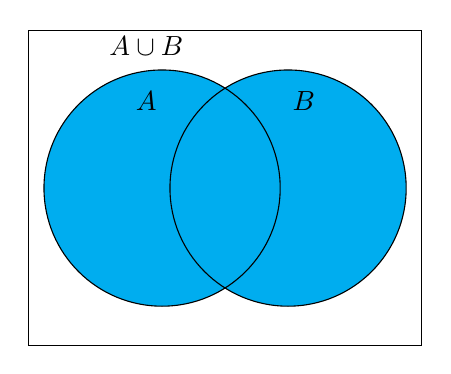
\begin{tikzpicture}
        \draw (-2.5,-2) rectangle (2.5,2);
        \fill[cyan] (-0.8cm,0) circle (1.5cm);
        \fill[cyan] (0.8cm,0) circle (1.5cm);
        \draw (-0.8cm,0) circle (1.5cm);
        \draw (0.8cm,0) circle (1.5cm);
        \node at (-1,1.1) {$A$};
        \node at (1,1.1) {$B$};
        \node at (-1,1.8) {$A\cup{B}$};
    \end{tikzpicture}
\end{document}
            \caption{Venn Diagram for Unions}
            \label{fig:Venn_Diagram_Union}
        \end{figure}
        \begin{lexample}{Union of Two Sets}{Union_of_Two_Sets}
            If we let $A$ and $B$ be defined as follows:
            \par
            \begin{subequations}
                \begin{minipage}[b]{0.49\textwidth}
                    \centering
                    \begin{equation}
                        A=\{\,3,\,5,\,6\,\}
                    \end{equation}
                \end{minipage}
                \hfill
                \begin{minipage}[b]{0.49\textwidth}
                    \centering
                    \begin{equation}
                        B=\{\,2,\,9,\,11,\,5\,\}
                    \end{equation}
                \end{minipage}
            \end{subequations}
            \par\vspace{2.5ex}
            We can form the union $A\cup{B}$ as follows:
            \begin{equation}
                A\cup{B}=\{\,2,\,3,\,5,\,6,\,9,\,11\,\}
            \end{equation}
            That is, the set of all elements in either $A$ or $B$, or both.
            We can do this construction with infinite sets as well:
            \par
            \begin{subequations}
                \begin{minipage}[b]{0.30\textwidth}
                    \centering
                    \begin{equation}
                        \mathbb{N}\cup\mathbb{Z}=\mathbb{Z}
                    \end{equation}
                \end{minipage}
                \hspace{0.03\textwidth}
                \begin{minipage}[b]{0.30\textwidth}
                    \centering
                    \begin{equation}
                        \mathbb{N}_{e}\cup\mathbb{N}_{o}=\mathbb{N}
                    \end{equation}
                \end{minipage}
                \hspace{0.03\textwidth}
                \begin{minipage}[b]{0.30\textwidth}
                    \centering
                    \begin{equation}
                        \mathbb{Q}\cup\mathbb{Z}=\mathbb{Q}
                    \end{equation}
                \end{minipage}
            \end{subequations}
            \par\vspace{2.5ex}
            Where $\mathbb{N}_{e}$, $\mathbb{N}_{o}$, $\mathbb{N}$,
            $\mathbb{Z}$, and $\mathbb{Q}$ denote the sets of even numbers,
            odd numbers, natural numbers, integers, and rational numbers,
            respectively,
        \end{lexample}
        \begin{axiom}[Axiom of the Power Set]
            \label{ax:Axiom_of_the_Power_Set}%
            If $A$ is a set, then there is a set $\mathcal{P}(A)$, called the
            power set, such that $x\in\mathcal{P}(A)$ if and only if
            $x\subseteq{A}$.
        \end{axiom}
        This axiom allows us to define the power set of any set.
        \begin{ldefinition}{Power Set}{Power_Set}
            The power set of a set $A$ is the set
            $\mathcal{P}(A)$ defined by:
            \begin{equation}
                \mathcal{P}(A)=\{\,B\,:\,B\subseteq{A}\,\}
            \end{equation}
            That is, $\mathcal{P}(A)$ is the set of all subsets of $A$.
        \end{ldefinition}
        \begin{theorem}
            \label{thm:Cartesian_Product_Exists}%
            If $A$ and $B$ are sets, then there is a set $C$ such that, for
            all $z$, $z\in{C}$ if and only if there exists $x\in{A}$ and
            $y\in{B}$ such that $z=(x,\,y)$.
        \end{theorem}
        \begin{proof}
            For let $\mathcal{O}=A\cup{B}$. Then by the axiom of the power set
            (Ax.~\ref{ax:Axiom_of_the_Power_Set}), the power set
            $\mathcal{P}(\mathcal{O})$ exists. But, again by the axiom of the
            power set, the power set
            $\mathcal{P}\big(\mathcal{P}(\mathcal{O})\big)$ exists. But then
            $z\in\mathcal{P}\big(\mathcal{P}(\mathcal{O})\big)$
            if and only if $z\subseteq\mathcal{P}(\mathcal{O})$, and for all
            $x\in{A}$ and $y\in{B}$,
            $(x,\,y)\subseteq\mathcal{P}(\mathcal{O})$. Let $P$ be the
            proposition $P(z)$ is true if and only if there exists $x\in{A}$
            and $y\in{B}$ such that $z=(x,\,y)$. Then, by the axiom schema of
            specification (Ax.~\ref{ax:Axiom_Schema_of_Specification}),
            there is a set $C$ such that:
            \begin{equation}
                C=\{\,z\,:\,P(z)\,\}
            \end{equation}
            Therefore, etc.
        \end{proof}
        The set $C$ constructed in Thm.~\ref{thm:Cartesian_Product_Exists} is
        the set of all ordered pairs of elements whose first entry is from the
        set $A$ and whose second entry comes from the set $B$. This is
        precisely the what we want the Cartesian product of $A$ with $B$ to
        be. Thus, this theorem gives justification to the following
        definition:
        \begin{ldefinition}{Cartesian Product}{Cartesian_Product}
            The \gls{Cartesian product} of a set $A$ with respect to a set
            $B$ is the set:
            \begin{equation}
                A\times{B}\equiv\{\;(a,\,b)\,:\,a\in{A}
                                    \textrm{ and }b\in{B}\;\}
            \end{equation}
            Where $(a,\,b)$ denotes the ordered pair of $a$ with $b$.
        \end{ldefinition}
        Much the way ordered pairs place order onto two arbitrary elements,
        Cartesian products place order on sets. Given two distinct sets $A$
        and $B$, we have that $A\times{B}\ne{B}\times{A}$, and thus the
        order in which we performed the Cartesian product is important. The
        validity of this statement stems from the fact that, in general,
        $(a,\,b)\ne(b,\,a)$, and thus if $A$ and $B$ are distinct sets they'll
        have at least some different elements, meaning $A\times{B}$ will have
        different ordered pairs than $B\times{A}$.
        \begin{lexample}{Cartesian Products}{Basic_Cartesian_Products}
            Let $A$ and $B$ be sets defined as follows:
            \par
            \begin{subequations}
                \begin{minipage}[b]{0.49\textwidth}
                    \centering
                    \begin{equation}
                        A=\{\,1,\,2,\,3\,\}
                    \end{equation}
                \end{minipage}
                \hfill
                \begin{minipage}[b]{0.49\textwidth}
                    \centering
                    \begin{equation}
                        B=\{\,a,\,b\,\}
                    \end{equation}
                \end{minipage}
            \end{subequations}
            \par\vspace{2.5ex}
            Let's compute $A\times{B}$ and $B\times{A}$. From the definition
            (Def.~\ref{def:Cartesian_Product}) we have:
            \begin{equation}
                A\times{B}=\{\;(a,b)\,:\,a\in{A}\textrm{ and }b\in{B}\;\}
            \end{equation}
            Using this, we can compute:
            \begin{equation}
                A\times{B}=\big\{\,(1,a),\,(2,a),\,(3,a),\,
                                   (1,b),\,(2,b),\,(3,b)\,\big\}
            \end{equation}
            Computing $B\times{A}$, we have:
            \begin{equation}
                B\times{A}=\big\{\,(a,\,1),\,(a,\,2),\,(a,\,3),\,
                                   (b,\,1),\,(b,\,2),\,(b,\,3)\,\big\}
            \end{equation}
            Now if we suppose that $a$ is not equal to 1, then we see that
            $(a,1)$ is a different element than $(1,a)$, and thus $A\times{B}$
            is not equal to $B\times{A}$. Next, compute $A\times{A}$:
            \begin{equation}
                A\times{A}=\big\{\,(1,1),\,(1,2),\,(1,3),\,
                                   (2,1),\,(2,2),\,(2,3),\,
                                   (3,1),\,(3,2),\,(3,3)\,\big\}
            \end{equation}
            And finally $B\times{B}$:
            \begin{equation}
                B\times{B}=\big\{\,(a,\,a),\,(a,\,b),
                                 \,(b,\,a),\,(b,\,b)\,\big\}
            \end{equation}
            Equality of $A\times{B}$ and $B\times{A}$ is achieved if and only
            if $A=B$, or if either set is the empty set.
        \end{lexample}
        Note that in Ex.~\ref{ex:Basic_Cartesian_Products}, the \textit{size}
        of the Cartesian product of two sets was simply the product of the
        number of elements of the constituent sets. That is, we see that $A$
        has three elements and $B$ has two elements, but also that
        $A\times{B}$ has six elements. Moreover, $A\times{A}$ has nine
        elements and $B\times{B}$ has four. This pattern holds for the
        Cartesian products of any two \textit{finite} sets.
        \par\hfill\par
        It is common to consider the Cartesian product of a set with itself.
        That is, given a set $A$, we are often interested in $A\times{A}$. We
        denote this by writing $A^{2}$. One such example is when we consider
        the set of real numbers, $\mathbb{R}$. The Cartesian product
        $\mathbb{R}^{2}$ is called the \textit{Euclidean Plane},
        or the \textit{Cartesian Plane}, after Euclid of Alexandria and
        Ren\'{e} Descartes. This is because $\mathbb{R}^{2}$ is used to model
        both planar geometry and analytical geometry, of which Euclid and
        Descartes were pioneers of, respectively. The term Cartesian products
        is in honor of Ren\'{e} Descartes, as well.
        \begin{lexample}{Plane Lattice}{Lattice_N_times_N}
            Consider $\mathbb{N}^{2}$, where $\mathbb{N}$ denotes the set of
            natural numbers (Eqn.~\ref{eqn:Natural_Numbers_Ellipses}), and
            $\mathbb{N}^{2}$ denotes the Cartesian product of this set with
            itself. We can visualize this by drawing a lattice of points in the
            plane (Fig.~\subref{fig:Lattice_Cart_Prod_of_N_with_N}).
        \end{lexample}
        \begin{lexample}{Cartesian Plane}{The_Plane_R_times_R}
            Let $\mathbb{R}$ denote the set of real numbers, and let
            $A=\mathbb{R}$ and $B=\mathbb{R}$. Then we have:
            \begin{equation}
                A\times{B}=\mathbb{R}\times\mathbb{R}\equiv\mathbb{R}^{2}
            \end{equation}
            Where the symbol $\equiv$ again means that $\mathbb{R}^{2}$ is
            defined by this expression. Using the definition of Cartesian
            products (Def.~\ref{def:Cartesian_Product}), we obtain:
            \begin{equation}
                \mathbb{R}^{2}=\{\;(x,y)\,:\,x\in\mathbb{R}
                                   \textrm{ and }y\in\mathbb{R}\;\}
            \end{equation}
            That is, $\mathbb{R}^{2}$ is the set of all ordered pairs of real
            numbers. The first term is called the $x$ coordinate, and
            similarly the second term is called the $y$ coordinate. This is
            used to model planar geometry (Fig.\subref{fig:Cartesian_Plane}).
        \end{lexample}
        \begin{figure}[H]
            \centering
            \begin{subfigure}[b]{0.49\textwidth}
                \centering
                \resizebox{\textwidth}{!}{
                    %--------------------------------Dependencies----------------------------------%
%   tikz                                                                       %
%       arrows.meta                                                            %
%-------------------------------Main Document----------------------------------%
\begin{tikzpicture}[%
    >=Latex,
    line width=0.2mm,
    line cap=round,
    font=\Large
]
    % Coordinates for the points.
    \coordinate (x) at (2.2, 0.0);
    \coordinate (y) at (0.0, 2.9);
    \coordinate (z) at (2.2, 2.9);

    % Draw a grid.
    \draw[style=help lines] (-0.3, -0.3) grid (7.9, 7.9);

    % Axes.
    \begin{scope}[thick]
        \draw[->] (-0.3, 0) to (8.4, 0) node [above] {$\mathbb{R}$};
        \draw[->] (0, -0.3) to (0, 8.4) node [right] {$\mathbb{R}$};
    \end{scope}

    % Draw dashed lines to the point.
    \begin{scope}[densely dashed]
        \draw (x) to (z);
        \draw (y) to (z);
    \end{scope}

    % Draw dots marking the various points.
    \draw[fill=black] (x) circle (0.6mm);
    \draw[fill=black] (y) circle (0.6mm);
    \draw[fill=black] (z) circle (0.6mm);

    % Label the points x, y, and the dot (x,y) in the plane.
    \node at (x) [below=0.1]     {$x$};
    \node at (y) [left=0.1]      {$y$};
    \node at (z) [above right]   {$(x,\,y)$};
\end{tikzpicture}%
                }
                \subcaption{The Cartesian Plane $\mathbb{R}^{2}$}
                \label{fig:Cartesian_Plane}
            \end{subfigure}
            \begin{subfigure}[b]{0.49\textwidth}
                \centering
                \resizebox{\textwidth}{!}{%
                    %--------------------------------Dependencies----------------------------------%
%   tikz                                                                       %
%       arrows.meta                                                            %
%-------------------------------Main Document----------------------------------%
\begin{tikzpicture}[%
    >=Latex,
    line width=0.2mm,
    line cap=round
]

    % Axes.
    \begin{scope}[thick, font=\Large]
        \draw[->] (0, 0) to (8.4, 0) node [above] {$\mathbb{N}$};
        \draw[->] (0, 0) to (0, 8.4) node [right] {$\mathbb{N}$};
    \end{scope}

    \foreach\x in{1, 2, 3, 4, 5, 6, 7, 8}{
        \foreach\y in{1, 2, 3, 4, 5, 6, 7, 8}{
            \draw[fill=black] (\x, \y) circle (0.2mm);
        }
        \draw (\x, -0.1) to (\x, 0.1) node [below=1ex] {$\x$};
        \draw (-0.1, \x) to (0.1, \x) node [left=1ex]  {$\x$};
    }
\end{tikzpicture}%
                }
                \caption{The Lattice $\mathbb{N}^{2}$}
                \label{fig:Lattice_Cart_Prod_of_N_with_N}
            \end{subfigure}
            \caption{Examples of Cartesian Products}
            \label{fig:Cartesian_Products_Examples}
        \end{figure}
        \begin{lexample}{}{Generic_Cartesian_Product}
            Consider the following sets:
            \par
            \begin{subequations}
                \begin{minipage}[b]{0.49\textwidth}
                    \centering
                    \begin{equation}
                        A=\{\,\textrm{Point, Line 1, Line 2}\,\}
                    \end{equation}
                \end{minipage}
                \hfill
                \begin{minipage}[b]{0.49\textwidth}
                    \centering
                    \begin{equation}
                        B=\{\,\textrm{Point, Line}\,\}
                    \end{equation}
                \end{minipage}
            \end{subequations}
            \par\vspace{2.5ex}
            We can visually represent the Cartesian product $A\times{B}$ by
            drawing $A$ in green and $B$ in red, as shown in
            Fig.~\ref{fig:Cartesian_Product_Example}. The Cartesian Product
            $A\times{B}$ is the set formed by connecting all of the points
            from $A$ and $B$ in the plane. This is shown in blue.
        \end{lexample}
        \begin{figure}[H]
            \centering
            %--------------------------------Dependencies----------------------------------%
%   tikz                                                                       %
%       arrows.meta                                                            %
%-------------------------------Main Document----------------------------------%
\begin{tikzpicture}[%
    >=Latex,
    line width=0.2mm,
    line cap=round
]

    % Draw green to indicate the set A.
    \begin{scope}[green]

        % Draw some points.
        \draw[fill=green] (1, 0) circle (0.3mm);
        \draw[fill=green] (2, 0) circle (0.3mm);
        \draw[fill=green] (5, 0) circle (0.3mm);
        \draw[fill=green] (6, 0) circle (0.3mm);
        \draw[fill=green] (7, 0) circle (0.3mm);

        % Draw lines.
        \draw (2, 0) to (5, 0);
        \draw (6, 0) to (7, 0);
    \end{scope}

    % Draw red to denote the set B.
    \begin{scope}[red]

        % Draw in some points.
        \draw[fill=red] (0, 1) circle (0.3mm);
        \draw[fill=red] (0, 2) circle (0.3mm);
        \draw[fill=red] (0, 5) circle (0.3mm);

        % Draw a line.
        \draw (0, 2) to (0, 5);
    \end{scope}

    % Use blue to mark AxB (Cartesian product).
    \begin{scope}[blue]

        % Fill in points.
        \draw[fill=blue] (1, 1) circle (0.3mm);
        \draw[fill=blue] (1, 2) circle (0.3mm);
        \draw[fill=blue] (1, 5) circle (0.3mm);
        \draw[fill=blue] (2, 1) circle (0.3mm);
        \draw[fill=blue] (5, 1) circle (0.3mm);
        \draw[fill=blue] (6, 1) circle (0.3mm);
        \draw[fill=blue] (7, 1) circle (0.3mm);
        \draw[fill=blue] (2, 2) circle (0.3mm);
        \draw[fill=blue] (2, 5) circle (0.3mm);
        \draw[fill=blue] (5, 2) circle (0.3mm);
        \draw[fill=blue] (5, 5) circle (0.3mm);
        \draw[fill=blue] (6, 2) circle (0.3mm);
        \draw[fill=blue] (7, 2) circle (0.3mm);
        \draw[fill=blue] (6, 5) circle (0.3mm);
        \draw[fill=blue] (7, 5) circle (0.3mm);

        % Draw lines.
        \draw (1, 2) to (1, 5);
        \draw (2, 1) to (5, 1);
        \draw (6, 1) to (7, 1);

        % Fill in rectangles.
        \draw[fill=blue, opacity=0.4] (2, 2) to (5, 2) to (5, 5)
                                             to (2, 5) to cycle;
        \draw[fill=blue, opacity=0.4] (6, 2) to (7, 2) to (7, 5)
                                             to (6, 5) to cycle;
        \draw (2, 2) to (5, 2) to (5, 5) to (2, 5) to cycle;
        \draw (6, 2) to (7, 2) to (7, 5) to (6, 5) to cycle;
    \end{scope}
\end{tikzpicture}
            \caption[Cartesian Product of Two Sets]
                {The Cartesian Product of Two Sets. $A$ is
                 in \textcolor{green}{Green},
                 $B$ is in \textcolor{red}{red}, and
                 $A\times{B}$ is in \textcolor{blue}{blue}.}
            \label{fig:Cartesian_Product_Example}
        \end{figure}
        Cartesian products are not \textit{associative}. That is, given three
        sets $A$, $B$, and $C$, there is no clear way to take the Cartesian
        product of these since:
        \begin{equation}
            A\times(B\times{C})\ne(A\times{B})\times{C}
        \end{equation}
        To see this, note that the elements of $A\times(B\times{C})$ are
        ordered pairs of the form $\big(a,\,(b,\,c)\big)$, whereas elements of
        $(A\times{B})\times{C}$ are of the form $\big((a,\,b),\,c\big)$. When
        we write $A\times{B}\times{C}$ we really want ordered \textit{triples}
        of the form $(a,\,b,\,c)$. Much the way ordered pairs have been
        defined, we can modify Kuratowski's approach and define ordered
        triples and ordered $n$ tuples. Rather than doing this we will use the
        language of functions to define higher order Cartesian products.
        \input{Chapters/Preliminaries/Set_Theory/The_Axiom_of_Choice.tex}
        \section{Operations on Sets}
        Similar to the arithmetic of real numbers, there
        are standard operations that can be performed on
        sets to obtain new sets. The four most common
        operations are union, intersection, set difference,
        and symmetric difference. Often the
        \textit{complement} of a set is discussed, but as
        we will see, this is just a specific case of set
        difference.
        \begin{figure}[H]
            \centering
            %--------------------------------Dependencies----------------------------------%
%   tikz                                                                       %
%-------------------------------Main Document----------------------------------%
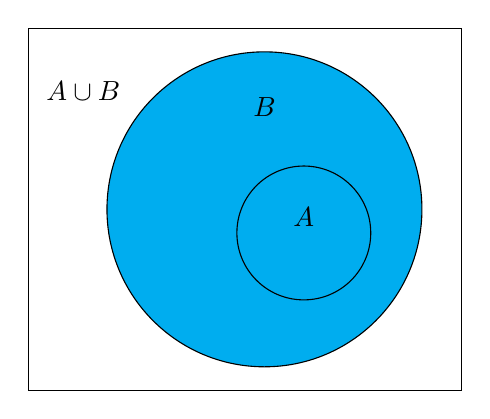
\begin{tikzpicture}
    \draw (-3,-2.3) rectangle (2.5,2.3);
    \draw[fill=cyan] (0,0) circle (2);
    \draw (0.5,-0.3) circle (0.85);

    \node at (0.5,-0.1) {$A$};
    \node at (0,1.3) {$B$};
    \node at (-2.3,1.5) {$A\cup{B}$};
\end{tikzpicture}
            \caption{Visual for Thm.~\ref{thm:Union_With_Subset}.}
            \label{fig:Venn_Diagram_Union_With_Subset}
        \end{figure}
        Set operations are very algebraic, and it is often
        useful to build up several small tools to eventually
        prove larger theorems in a simple way. We wish to
        show that union is commutative and associative, and
        that there is an \textit{identity}.
        \begin{ltheorem}{Commutative Law of Unions}{Commutative_Law_of_Unions}
            If $A$ and $B$ are sets, then $A\cup{B}=B\cup{A}$.
        \end{ltheorem}
        \begin{proof}
            For if $x\in{A}\cup{B}$, then either $x\in{A}$ or $x\in{B}$, or
            both (Def.~\ref{def:Union_of_Two}). But then either $x\in{B}$ or
            $x\in{A}$, or both, and therefore $x\in{B}\cup{A}$
            (Def.~\ref{def:Union_of_Two}). But then for all $x\in{A}\cup{B}$
            it is true that $x\in{B}\cup{A}$, and therefore
            $A\cup{B}\subseteq{B}\cup{A}$ (Def.~\ref{def:Subsets}). Similarly,
            $B\cup{A}\subseteq{A}\cup{B}$, and thus $A\cup{B}=B\cup{A}$
            (Def.~\ref{def:Equal_Sets}). Therefore, etc.
        \end{proof}
        When taking the union of two sets, we obtain a
        \textit{larger} set, in a sense. Again relying on
        the analogy of arithmetic, given two non-negative
        integers $a$ and $b$, it is true that $a\leq{a}+b$.
        Equality is obtained if and only if either $a$ or
        $b$ is equal to zero. As we will see, the empty set
        acts as the \textit{zero} of unions. Also, given
        three non-negative integers $a$, $b$, and $c$, if
        $b\leq{c}$, then $a+b\leq{a}+c$. A similar result
        will hold for sets and unions.
        \begin{theorem}
            \label{thm:Union_is_Bigger}%
            If $A$ and $B$ are sets, then
            $A\subseteq{A}\cup{B}$.
        \end{theorem}
        \begin{proof}
            For suppose not. Then there is an $x\in{A}$ such
            that $x\notin{A}\cup{B}$. But if $x\in{A}$, then
            $x\in{A}$ or $x\in{B}$ and thus $x\in{A}\cup{B}$
            (Def.~\ref{def:Union_of_Two}), a
            contradiction. Therefore, etc.
        \end{proof}
        \begin{theorem}
            \label{thm:Union_With_Lesser_Set}%
            If $A$, $B$, and $C$ are sets, and if
            $B\subseteq{C}$, then
            $A\cup{B}\subseteq{A}\cup{C}$.
        \end{theorem}
        \begin{proof}
            For if $x\in{A}\cup{B}$, then either $x\in{A}$,
            or $x\in{B}$, or both
            (Def.~\ref{def:Union_of_Two}). But $B$ is a
            subset of $C$, and therefore if $x\in{B}$, then
            $x\in{C}$ (Def.~\ref{def:Subsets}).
            Thus, if $x\in{A}$ or $x\in{B}$, then
            $x\in{A}$ or $x\in{C}$, and therefore
            $x\in{A}\cup{C}$ (Def.~\ref{def:Union_of_Two}).
            Thus, $A\cup{B}\subseteq{A}\cup{C}$
            (Def.~\ref{def:Subsets}). Therefore, etc.
        \end{proof}
        \begin{theorem}
            If $A$, $B$, $C$, and $D$ are sets, if
            $A\subseteq{C}$, and if $B\subseteq{D}$, then
            $A\cup{B}\subseteq{C}\cup{D}$.
        \end{theorem}
        \begin{proof}
            For if $B\subseteq{D}$, then
            $A\cup{B}\subseteq{A}\cup{D}$
            (Thm.~\ref{thm:Union_With_Lesser_Set}).
            But $A\cup{D}=D\cup{A}$
            (Thm.~\ref{thm:Commutative_Law_of_Unions}).
            But if $A\subseteq{C}$, then
            $D\cup{A}\subseteq{D}\cup{C}$
            (Thm.~\ref{thm:Union_With_Lesser_Set}). But
            $D\cup{C}=C\cup{D}$
            (Thm.~\ref{thm:Commutative_Law_of_Unions}).
            And if $A\cup{B}\subseteq{A}\cup{D}$ and
            $A\cup{D}\subseteq{C}\cup{D}$, then
            $A\cup{B}\subseteq{C}\cup{D}$
            (Thm.~\ref{thm:Subset_is_Transitive}).
            Therefore, etc.
        \end{proof}
        Taking the union of subsets is redundant, as we
        simply obtain the larger set. This starts to break
        down the analogy between sets and arithmetic, since
        there is only one \textit{zero}. That is, there is
        only one number $b$ such that $a+b=a$, and that is
        $b=0$. While any subset acts as a \textit{zero} of a
        given set, the empty set has the property that it
        acts as a zero for \textit{every} set. It is the only
        set with this property, and thus the analogy with
        arithmetic is restored.
        \begin{theorem}
            \label{thm:Union_With_Subset}%
            If $A$ and $B$ are sets, and if
            $A\subseteq{B}$, then $A\cup{B}=B$.
        \end{theorem}
        \begin{proof}
            For if $A$ and $B$ are sets, then
            $B\subseteq{A}\cup{B}$
            (Thm.~\ref{thm:Union_is_Bigger}).
            But if $A\subseteq{B}$, then for all $x\in{A}$,
            it is true that $x\in{B}$
            (Def.~\ref{def:Subsets}). Thus if $x\in{A}$ or if
            $x\in{B}$, then $x\in{B}$. But then, for all
            $x\in{A}\cup{B}$, it is true that $x\in{B}$, and
            therefore $A\cup{B}\subseteq{B}$
            (Def.~\ref{def:Subsets}). Thus,
            $A\cup{B}=B$ (Def.~\ref{def:Equal_Sets}).
            Therefore, etc.
        \end{proof}
        \begin{theorem}
            \label{thm:Union_with_Emptyset}%
            If $A$ is a set, then $A=\emptyset\cup{A}$.
        \end{theorem}
        \begin{proof}
            For $\emptyset\subseteq{A}$
            (Thm.~\ref{thm:Emptyset_Is_Subset}) and
            therefore $\emptyset\cup{A}=A$
            (Thm.~\ref{thm:Union_With_Subset}).
        \end{proof}
        \begin{theorem}
            \label{thm:Empty_Set_Is_Zero_for_Unions}%
            If $A$ is a set such that, for any set $B$, it is
            true that $A\cup{B}=B$, then $A$ is the
            empty set.
        \end{theorem}
        \begin{proof}
            For suppose not. If $A\ne\emptyset$, then there
            is an $x\in{A}$ (Def.~\ref{def:Empty_Set}).
            But then $B=\{A\}$ is a set
            (Def.~\ref{def:Sets}). But then $x\in{A}\cup{B}$
            (Def.~\ref{def:Union_of_Two}). But $x\notin{B}$,
            and thus $A\cup{B}\ne{B}$
            (Def.~\ref{def:Equal_Sets}), a contradiction
            since $A$ is such that for any set $B$, it is
            true that $A\cup{B}=B$. Therefore, etc.
        \end{proof}
        Thm.~\ref{thm:Empty_Set_Is_Zero_for_Unions} proves
        the assertion that the empty set is the zero of set
        union. The converse of
        Thm.~\ref{thm:Union_With_Subset} can be proved as
        well.
        \begin{theorem}
            \label{thm:Conv_Union_Is_Bigger}%
            If $A$ and $B$ are sets, and if
            $A\cup{B}\subseteq{A}$, then $A\cup{B}=A$.
        \end{theorem}
        \begin{proof}
            For $A\subseteq{A}\cup{B}$
            (Thm.~\ref{thm:Union_is_Bigger}). But by
            hypothesis, $A\cup{B}\subseteq{A}$. But then
            $A=A\cup{B}$ (Def.~\ref{def:Equal_Sets}).
            Therefore, etc.
        \end{proof}
        \begin{theorem}
            \label{thm:Union_is_Equal}%
            If $A$ and $B$ are sets, and if
            $A\cup{B}\subseteq{A}$, then $B\subseteq{A}$.
        \end{theorem}
        \begin{proof}
            For if $A\cup{B}\subseteq{A}$, then
            $A\cup{B}=A$
            (Thm.~\ref{thm:Conv_Union_Is_Bigger}). And also,
            $B\subseteq{A}\cup{B}$
            (Thm.~\ref{thm:Union_is_Bigger}). But if
            $A\cup{B}=A$ and $B\subseteq{A}\cup{B}$, then
            $B\subseteq{A}$
            (Thm.~\ref{thm:Subsets_of_Equal_Sets}).
            Therefore, etc.
        \end{proof}
        We'll wrap up unions by showing that the operation
        is associative. Once again relying on the analogy
        of arithmetic, given three real numbers $a$, $b$,
        and $c$, it is true that $a+(b+c)=(a+b)+c$. This
        is called the associative law of addition. Combining
        this law with the commutative law shows that the
        order in which three real numbers are added is
        irrelevant. Applying induction, we see that given
        any finite collection of real numbers, the order in
        which we add them is again irrelevant. The same holds
        true for the union of sets.
        \begin{theorem}
            \label{thm:First_Assoc_Law_Union}%
            If $A$, $B$, and $C$ are sets, then
            $A\cup(B\cup{C})\subseteq(A\cup{B})\cup{C}$.
        \end{theorem}
        \begin{proof}
            For $B\subseteq{A}\cup{B}$
            (Thm.~\ref{thm:Union_is_Bigger}), and thus
            $B\cup{C}\subseteq(A\cup{B})\cup{C}$
            (Thm.~\ref{thm:Union_With_Lesser_Set}). But then
            $A\cup(B\cup{C})\subseteq{A}%
             \cup((A\cup{B})\cup{C})$
            (Thm.~\ref{thm:Union_With_Lesser_Set}).
            But $A\subseteq{A}\cup{B}$ and
            $A\cup{B}\subseteq(A\cup{B})\cup{C}$
            (Thm.~\ref{thm:Union_is_Bigger}), and therefore
            $A\subseteq(A\cup{B})\cup{C}$
            (Thm.~\ref{thm:Subset_is_Transitive}). But then
            $(A\cup)B\cup{C}={A}\cup((A\cup{B})\cup{C})$
            (Thm.~\ref{thm:Union_With_Subset}). But it was
            proved that
            $A\cup(B\cup{C})\subseteq{A}%
             \cup((A\cup{B})\cup{C})$, and therefore
            $A\cup(B\cup{C})\subseteq(A\cup{B})\cup{C}$
            (Thm.~\ref{thm:Subsets_of_Equal_Sets}).
            Therefore, etc.
        \end{proof}
        \begin{ltheorem}{Associative Law of Unions}
              {Associative_Law_of_Unions}
            If $A$, $B$, and $C$ are sets, then
            $A\cup(B\cup{C})=(A\cup{B})\cup{C}$.
        \end{ltheorem}
        \begin{proof}
            For by the Commutative Law of Unions
            (Thm.~\ref{thm:Commutative_Law_of_Unions}),
            we have:
            \begin{equation}
                (A\cup{B})\cup{C}=C\cup(A\cup{B})
                                 =C\cup(B\cup{A})
            \end{equation}
            But $C\cup(B\cup{A})\subseteq(C\cup{B})\cup{A}$
            (Thm.~\ref{thm:First_Assoc_Law_Union}). Again by
            commutativity, we obtain:
            \begin{equation}
                (C\cup{B})\cup{A}=A\cup(C\cup{B})
                                 =A\cup(B\cup{C})
            \end{equation}
            Therefore,
            $(A\cup{B})\cup{C}\subseteq{A}\cup(B\cup{C})$.
            But $A\cup(B\cup{C})\subseteq(A\cup{B})\cup{C}$
            (Thm.~\ref{thm:First_Assoc_Law_Union}),
            and thus $A\cup(B\cup{C})=(A\cup{B})\cup{C}$
            (Def.~\ref{def:Equal_Sets}). Therefore, etc.
        \end{proof}
        \begin{theorem}
            \label{thm:Redundant_Union}%
            If $A$, $B$, and $C$ are sets and if
            $A\subseteq{B}$, then
            $A\cup(B\cup{C})=B\cup{C}$
        \end{theorem}
        \begin{proof}
            For $B\cup{C}\subseteq{A}\cup(B\cup{C})$
            (Thm.~\ref{thm:Union_is_Bigger}). But
            $A\cup(B\cup{C})=(A\cup{B})\cup{C}$
            (Thm.~\ref{thm:Associative_Law_of_Unions}).
            And since $A$ is a subset of $B$,
            $A\cup{B}=B$ (Thm.~\ref{thm:Union_With_Subset}),
            and thus $(A\cup{B})\cup{C}=B\cup{C}$. Thus,
            $B\cup{C}=A\cup(B\cup{C})$
            (Thm.~\ref{thm:Equality_Transitive}).
            Therefore, etc.
        \end{proof}
        \begin{ldefinition}{Intersection of Two Sets}
              {Intersection_of_Two}
            The intersection of two sets $A$ and $B$,
            denoted $A\cap{B}$, is the set:
            \begin{equation}
                A\cap{B}
                =\{\;x\,:\,x\in{A}\textrm{ and }x\in{B}\;\}
            \end{equation}
            That is, the set of elements $x$ that are in
            both $A$ and $B$.
        \end{ldefinition}
        Similar to set union, intersections can be visualized
        by Venn diagrams. See
        Fig.~\ref{fig:Union_Intersection_venn_diagram}.
        \begin{figure}[H]
            \centering
            \captionsetup{type=figure}
            \documentclass[crop,class=article]{standalone}
%----------------------------Preamble-------------------------------%
\usepackage{tikz}                       % Drawing/graphing tools.
%--------------------------Main Document----------------------------%
\begin{document}
    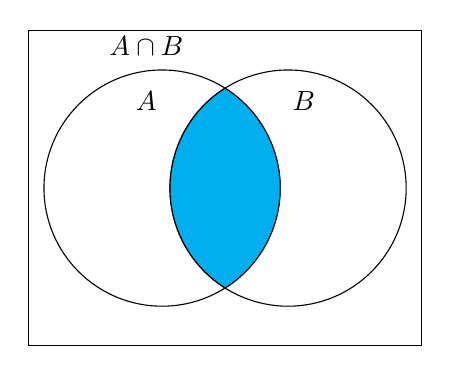
\begin{tikzpicture}
        \draw (-2.5,-2) rectangle (2.5,2);
        \draw (-0.8cm,0) circle (1.5cm);
        \draw (0.8cm,0) circle (1.5cm);
        \draw[fill=cyan]
            (0,-1.26886) arc(-57.77:57.77:1.5)
                         arc(122.231:237.7690:1.5);
        \node at (-1,1.1) {$A$};
        \node at (1,1.1) {$B$};
        \node at (-1,1.8) {$A\cap{B}$};
    \end{tikzpicture}
\end{document}
            \caption{Venn Diagrams for Intersections}
            \label{fig:Union_Intersection_venn_diagram}
        \end{figure}
        \begin{ltheorem}{Commutative Law of Intersections}
                        {Commut_Law_Intersec}
            If $A$ and $B$ are sets, then $A\cap{B}=B\cap{A}$.
        \end{ltheorem}
        \begin{proof}
            For if $x\in{A}\cap{B}$, then $x\in{A}$ and
            $x\in{B}$. But then $x\in{B}$ and $x\in{A}$,
            and therefore $x\in{B}\cap{A}$
            (Def.~\ref{def:Intersection_of_Two}). But then
            for all $x\in{A}\cap{B}$ it is true that
            $x\in{B}\cap{A}$, and therefore
            $A\cup{B}\subseteq{B}\cup{A}$
            (Def.~\ref{def:Subsets}). Similarly,
            $B\cap{A}\subseteq{A}\cap{B}$, and thus
            $A\cap{B}=B\cap{A}$ (Def.~\ref{def:Equal_Sets}).
            Therefore, etc.
        \end{proof}
        \begin{theorem}
            \label{thm:Intersection_is_Smaller}%
            If $A$ snd $B$ are sets, then
            $A\cap{B}\subseteq{A}$.
        \end{theorem}
        \begin{proof}
            If $x\in{A}\cap{B}$, then $x\in{A}$ and
            $x\in{B}$, and thus $x\in{A}$. Therefore, etc.
        \end{proof}
        \begin{theorem}
            \label{thm:Intersection_with_Lesser_Set}%
            If $A$, $B$, and $C$ are sets, and if
            $B\subseteq{C}$, then
            $A\cap{B}\subseteq{A}\cap{C}$.
        \end{theorem}
        \begin{proof}
            For if $x\in{A}\cap{B}$, then $x\in{A}$ and
            $x\in{B}$ (Def.~\ref{def:Intersection_of_Two}).
            But $B$ is a subset of $C$, and thus if
            $x\in{B}$, then $x\in{C}$
            (Def.~\ref{def:Subsets}). But then $x\in{A}$ and
            $x\in{C}$, and therefore $x\in{A}\cap{C}$
            (Def.~\ref{def:Intersection_of_Two}). But
            then $A\cap{B}\subseteq{A}\cap{C}$
            (Def.~\ref{def:Subsets}). Therefore, etc.
        \end{proof}
        \begin{theorem}
            \label{thm:Intersection_is_Equal}%
            If $A$ and $B$ are sets, and if
            $A=A\cap{B}$, then $A\subseteq{B}$.
        \end{theorem}
        \begin{proof}
            For suppose not. Then there is an $x\in{A}$ such
            that $x\notin{B}$. But since $A=A\cap{B}$,
            if $x\in{A}$ then $x\in{A}\cap{B}$
            (Def.~\ref{def:Equal_Sets}). But if
            $x\in{A}\cap{B}$, then $x\in{B}$
            (Thm.~\ref{thm:Intersection_is_Smaller}),
            a contradiction. Therefore, etc.
        \end{proof}
        \begin{theorem}
            \label{thm:Intersection_of_Subset}%
            If $A$ and $B$ are sets, and if
            $A\subseteq{B}$, then $A\cap{B}=A$.
        \end{theorem}
        \begin{proof}
            For $A\cap{B}\subseteq{A}$
            (Thm.~\ref{thm:Intersection_is_Smaller}). But
            since $A$ is a subset of $B$, if $x\in{A}$, then
            $x\in{B}$ (Def.~\ref{def:Subsets}). But then
            $x\in{A}\cap{B}$
            (Def.~\ref{def:Intersection_of_Two}). Therefore,
            $A\subseteq{A}\cap{B}$ (Def~\ref{def:Subsets})
            and thus $A=A\cap{B}$ (Def~\ref{def:Equal_Sets}).
            Therefore, etc.
        \end{proof}
        \begin{theorem}
            \label{thm:Conv_Intersection_is_Smaller}%
            If $A$ and $B$ are sets, and if
            $A\subseteq{A}\cap{B}$, then $A=A\cap{B}$.
        \end{theorem}
        \begin{proof}
            For $A\cap{B}\subseteq{A}$
            (Thm.~\ref{thm:Intersection_is_Smaller}). But
            by hypothesis, $A\subseteq{A}\cap{B}$, and thus
            $A=A\cap{B}$ (Def.~\ref{def:Equal_Sets}).
            Therefore, etc.
        \end{proof}
        \begin{theorem}
            If $A$ is a set, then
            $\emptyset\cap{A}=\emptyset$.
        \end{theorem}
        \begin{proof}
            For $\emptyset\subseteq{A}$
            (Thm.~\ref{thm:Emptyset_Is_Subset}), and
            therefore $\emptyset\cap{A}=\emptyset$
            (Thm.~\ref{thm:Intersection_of_Subset}).
        \end{proof}
        \begin{theorem}
            \label{thm:First_Assoc_Law_Intersec}%
            If $A$, $B$, and $C$ are sets, then
            $A\cap(B\cap{C})\subseteq(A\cap{B})\cap{C}$.
        \end{theorem}
        \begin{proof}
            For if $x\in{A}\cap(B\cap{C})$, then $x\in{A}$
            and $x\in{B}\cap{C}$
            (Def.~\ref{def:Intersection_of_Two}). But if
            $x\in{B}\cap{C}$, then $x\in{B}$ and $x\in{C}$
            (Def.~\ref{def:Intersection_of_Two}). But then
            $x\in{A}$ and $x\in{B}$, and therefore
            $x\in{A}\cap{B}$
            (Def.~\ref{def:Intersection_of_Two}). But
            then $x\in{A}\cap{B}$ and $x\in{C}$, and
            therefore $x\in(A\cap{B})\cap{C}$
            (Def.~\ref{def:Intersection_of_Two}). Thus,
            $A\cap(B\cap{C})\subseteq(A\cap{B})\cap{C}$
            (Def.~\ref{def:Subsets}). Therefore, etc.
        \end{proof}
        \begin{ltheorem}{Associative Law of Intersections}
              {Assoc_Law_Intersec}
            If $A$, $B$, and $C$ are sets, then
            $A\cap(B\cap{C})=(A\cap{B})\cap{C}$.
        \end{ltheorem}
        \begin{proof}
            For by the Commutative Law of Intersections
            (Thm.~\ref{thm:Commut_Law_Intersec}),
            we have:
            \begin{equation}
                (A\cap{B})\cap{C}=C\cap(A\cap{B})
                                 =C\cap(B\cap{A})
            \end{equation}
            But $C\cap(B\cap{A})\subseteq(C\cap{B})\cap{A}$
            (Thm.~\ref{thm:First_Assoc_Law_Intersec}).
            Again by commutativity, we obtain:
            \begin{equation}
                (C\cap{B})\cap{A}=A\cap(C\cap{B})
                                 =A\cap(B\cap{C})
            \end{equation}
            Therefore,
            $(A\cap{B})\cap{C}\subseteq{A}\cap(B\cap{C})$.
            But $A\cap(B\cap{C})\subseteq(A\cap{B})\cap{C}$
            (Thm.~\ref{thm:First_Assoc_Law_Intersec}),
            and thus $A\cap(B\cap{C})=(A\cap{B})\cap{C}$
            (Def.~\ref{def:Equal_Sets}). Therefore, etc.
        \end{proof}
        \begin{theorem}
            \label{thm:Redundant_Intersection}%
            If $A$, $B$, and $C$ are sets and if
            $B\subseteq{A}$, then
            $A\cap(B\cap{C})=B\cap{C}$.
        \end{theorem}
        \begin{proof}
            For $A\cup(B\cup{C})\subseteq{B}\cup{C}$
            (Thm.~\ref{thm:Intersection_is_Smaller}). But
            $A\cap(B\cap{C})=(A\cap{B})\cap{C}$
            (Thm.~\ref{thm:Assoc_Law_Intersec}).
            And since $B$ is a subset of $A$,
            $A\cap{B}=A$
            (Thm.~\ref{thm:Intersection_of_Subset}),
            and thus $(A\cap{B})\cap{C}=B\cap{C}$. Thus,
            $B\cap{C}=A\cap(B\cap{C})$
            (Thm.~\ref{thm:Equality_Transitive}).
            Therefore, etc.
        \end{proof}
        \begin{theorem}
            \label{thm:First_Pseudo_Dist_Law_Union}%
            If $A$, $B$, and $C$ are sets, then
            $(B\cap{C})\subseteq(A\cup{B})\cap(A\cup{C})$.
        \end{theorem}
        \begin{proof}
            For $B\subseteq{A}\cup{B}$
            (Thm.~\ref{thm:Union_is_Bigger}). But then
            $B\cap{C}\subseteq(A\cup{B})\cap{C}$
            (Thm.~\ref{thm:Intersection_with_Lesser_Set}).
            But $C\subseteq{A}\cup{C}$
            (Thm.~\ref{thm:Union_is_Bigger}), and thus
            $(A\cup{B})\cap{C}%
             \subseteq(A\cup{B})\cap{A}\cup{C}$
            (Thm.~\ref{thm:Intersection_with_Lesser_Set}).
            But it was just proved that
            $B\cap{C}\subseteq(A\cup{B})\cap{C}$, and
            therefore by transivity,
            $(B\cap{C})\subseteq(A\cup{B})\cap(A\cup{C})$
            (Thm.~\ref{thm:Subset_is_Transitive}).
            Therefore, etc.
        \end{proof}
        \begin{ltheorem}{Distributive Law of Unions}
              {Distributive_Law_Union}
            If $A$, $B$, and $C$ are sets, then
            $A\cup(B\cap{C})=(A\cup{B})\cap(A\cup{C})$.
        \end{ltheorem}
        \begin{proof}
            For $(B\cap{C})\subseteq(A\cup{B})\cap(A\cup{C})$
            (Thm.~\ref{thm:First_Pseudo_Dist_Law_Union}).
            But then:
            \begin{equation}
                A\cup(B\cap{C})\subseteq
                A\cup\Big((A\cup{B})\cap(A\cup{C})\Big)
            \end{equation}
            But $A\cup((A\cup{B})\cap(A\cup{C}))%
                 =(A\cup{B})\cap(A\cup{C})$, and therefore:
            \begin{equation}
                A\cup(B\cap{C})\subseteq
                (A\cup{B})\cap(A\cup{C})
            \end{equation}
        \end{proof}
        \begin{ltheorem}{Distributive Law of Intersections}
              {Distributive_Law_Intersections}
            If $A$, $B$, and $C$ are sets, then
            $A\cap(B\cup{C})=(A\cap{B})\cup(A\cap{C})$.
        \end{ltheorem}
        \begin{proof}
            Hi
        \end{proof}
        If $A$ and $B$ are sets, and if
        $C\subseteq{A}\cup{B}$, then
        either $C\subseteq{A}$ or $C\subseteq{B}$, or both.
        It is possible that $C\subseteq{A}\cup{B}$ and yet
        $C$ and $B$ have no elements in common, as long
        as $C\subseteq{A}$. As an example,
        take $A$ and $B$ to be disjoint sets. Then
        $A\subseteq{A}\cup{B}$, yet $A$ and $B$ have no
        elements in common. If $C\subseteq{A}\cap{B}$, then
        it must be true that $C\subseteq{A}$ and
        $C\subseteq{B}$.
        Using arithmetic as an analogy, the empty set
        acts somewhat like a zero element. It is an identity
        element under set unions, and collapses everything
        down to zero under set intersections. Continuing
        with this analogy, we discuss set difference.
        \begin{ldefinition}{Set Difference}{Set_Difference}
            The set difference of a set $A$ with respect to
            a set $B$, denoted $B\setminus{A}$, is the set:
            \begin{equation}
                B\setminus{A}=\{x\in{B}:x\notin{A}\}
            \end{equation}
        \end{ldefinition}
        \begin{ldefinition}{Symmetric Difference}
              {Symmetric_Difference}
            The symmetric difference of $A$ and $B$, denoted
            $A\ominus{B}$, is the set:
            \begin{equation}
                A\ominus{B}
                =(A\cup{B})\setminus(A\cap{B})
            \end{equation}
        \end{ldefinition}
        While set difference appears similar to subtraction,
        the two have their differences. For any two real
        numbers $a$ and $b$, it is always true that
        $b=a-(a-b)$. For sets this is not true. For let $A$
        be the empty set, and let $B$ be non-empty.
        Then $A\setminus(A\setminus{B})=\emptyset$, which
        is not $B$. Set differences can not be easily
        simplified. The notion is not associative, nor is it
        commutative. If there is a larger \textit{universe}
        set, then set difference can be related to
        intersection.
        \begin{theorem}
            \label{thm:Set_Difference_As_Intersection}%
            If $A$, $B$, and $C$ are sets, and if
            $A\subseteq{C}$ and $B\subseteq{C}$, then:
            \begin{equation}
                B\setminus{A}=B\cap(C\setminus{A})
            \end{equation}
        \end{theorem}
        \begin{proof}
            For if $x\in{B}\setminus{A}$, then
            $x\in{B}$ and $x\notin{A}$. But
            $B\subseteq{C}$, and thus if $x\in{B}$, then
            $x\in{C}$. But if $x\notin{A}$, then
            $x\in{C}\setminus{A}$. Therefore
            $B\setminus{A}\subseteq{B}\cap(C\setminus{A})$.
            Similarly,
            $B\cap(C\setminus{A})\subseteq{B}\setminus{A}$,
            and therefore
            $B\setminus{A}={B}\cap(C\setminus{A})$.
        \end{proof}
        Similar to unions and intersections,
        set differences and symmetric differences can be
        visualized by Venn diagrams, as shown in
        Fig.~\ref{fig:Difference_Sym_Venn_Diagram}.
        \begin{figure}[H]
            \centering
            \caption{Caption}
            \label{fig:Difference_Sym_Venn_Diagram}
        \end{figure}
        The concept of set difference can then be used to
        define the concept of complement.
        \begin{ldefinition}{Complement}{Complement}
            The complement of a set $A$ with respect to a set
            $\Omega$, denoted $A^{C}$, is the set:
            \begin{equation}
                A^{C}=\Omega\setminus{A}
            \end{equation}
        \end{ldefinition}
        Thm.~\ref{thm:Set_Difference_As_Intersection}
        can then be translated into the notation of
        complements as follows:
        \begin{theorem}
            If $A$, $B$, and $\Omega$ are sets,
            $A,B\subseteq\Omega$, and if $A^{C}$ is the
            complement of $A$ with respect to $\Omega$, then:
            \begin{equation}
                B\setminus{A}=B\cap{A}^{C}
            \end{equation}
        \end{theorem}
        \begin{proof}
            By the definition of complement,
            $A^{C}=\Omega\setminus{A}$.
            As $A\subseteq\Omega$ and $B\subseteq\Omega$, by
            Thm.~\ref{thm:Set_Difference_As_Intersection},
            $B\setminus{A}=B\cap(\Omega\setminus{A})$,
            and therefore $B\setminus{A}=B\cap{A}^{C}$.
        \end{proof}
        The main result about complements are known as
        DeMorgan's Laws. The laws relate unions and
        intersections by means of complements. The general
        laws hold for arbitrary unions and arbitrary
        intersections, as will be shown later.
        \begin{ftheorem}{DeMorgan's Laws}{MEASURE_DEMORGAN}
            If $A$, $B$, and $\Omega$ are sets, if
            $A\subseteq\Omega$ and $B\subseteq\Omega$, then:
            \begin{subequations}
                \begin{align}
                    \big(A\cap{B}\big)^{C}
                        &=A^{C}\cup{B}^{C}\\
                    \big(A\cup{B}\big)^{C}
                        &=A^{C}\cap{B}^{C}
                \end{align}
            \end{subequations}
        \end{ftheorem}
        \begin{proof}
            It do.
        \end{proof}
        With this, we can prove some results about
        set differences.
        \begin{theorem}
            If $A$ and $B$ are sets, then:
            \begin{equation}
                A=\big(A\cap{B}\big)
                    \cup\big(A\setminus{B}\big)
            \end{equation}
        \end{theorem}
        \begin{proof}
            For let $\Omega=A\cup{B}$. Then
            $A\subseteq\Omega$ and $B\subseteq\Omega$,
            and thus:
            \begin{subequations}
                \begin{align}
                    \big(A\cap{B})\cup\big(A\setminus{B}\big)
                    &=\big(A\cap{B}\big)
                        \cup\big(A\cap{B}^{C}\big)\\
                    &=A\cap(B\cup{B}^{C})\\
                    &=A\cap\Omega
                \end{align}
            \end{subequations}
            But by Thm.~\ref{thm:Intersection_is_Smaller},
            $A\cap\Omega=A$. Therefore, etc.
        \end{proof}
        \begin{theorem}
            If $A$, $B$, and $C$ are sets, then:
            \begin{equation}
                A\cap\big(B\setminus{C}\big)
                =\big(A\cap{B}\big)\cap\big(A\setminus{C}\big)
            \end{equation}
        \end{theorem}
        \begin{proof}
            For:
            \begin{subequations}
                \begin{align}
                    A\cap\big(B\setminus{C}\big)
                    &=A\cap\big(B\cap{C}^{C}\big)\\
                    &=\big(A\cap{A}\big)
                        \cap\big(B\cap{C}^{C}\big)\\
                    &=\big(A\cap{B}\big)
                        \cap\big(A\cap{C}^{C}\big)\\
                    &=\big(A\cap{B}\big)
                        \cap\big(A\setminus{C}\big)
                \end{align}
            \end{subequations}
        \end{proof}
        Intersections do distribute over set differences.
        \begin{theorem}
            If $A$, $B$, and $C$ are sets, then:
            \begin{equation}
                A\cap(B\setminus{C})=
                (A\cap{B})\setminus(A\cap{C})
            \end{equation}
        \end{theorem}
        \begin{proof}
            For:
            \begin{subequations}
                \begin{align}
                    \big(A\cap{B}\big)\setminus
                        \big(A\cap{C}\big)
                    &=\big(A\cap{B}\big)
                        \cap\big(A\cap{C}\big)^{C}\\
                    &=\big(A\cap{B}\big)
                        \cap\big(A^{C}\cup{C}^{C}\big)\\
                    &=\big[\big(A\cap{B}\big)\cap{A}^{C}\big]
                        \cup\big[\big({A}\cap{B}\big)
                        \cap{C}^{C}\big]\\
                    &=\big[\big(A\cap{A}^{C}\big)\cap{B}\big]
                        \cup\big[\big(A\cap{B}\big)
                        \cap{C}^{C}\big]\\
                    &=\emptyset\cup\big[\big(A\cap{B}\big)
                        \cap{C}^{C}\big]\\
                    &=\big(A\cap{B}\big)\cap{C}^{C}\\
                    &=A\cap\big(B\cap{C}^{C}\big)\\
                    &=A\cap\big(B\setminus{C}\big)
                \end{align}
            \end{subequations}
            Therefore, etc.
        \end{proof}
        Unions do not, however. For let $A$ be non-empty
        and let $A=B=C$. Then $A\cup(B\setminus{C})=A$, but
        $(A\cup{B})\setminus(A\cup{C})=\emptyset$.
        DeMorgan's Laws hold for arbitrary collections
        of set. If $I$ is some indexing set:
        \begin{align}
            \Big(\bigcup_{\alpha\in{I}}A_{\alpha}\Big)^{C}
            &=\bigcap_{\alpha\in{I}}A_{\alpha}^{C}\\
            \Big(\bigcap_{\alpha\in{I}}A_{\alpha}\Big)^{C}
            &=\bigcup_{\alpha\in{I}}A_{\alpha}^{C}
        \end{align}
        The set operations thus define binary operations
        on the power set of a set $\Omega$. It's important
        to note the notation. An element of $\Omega$ may
        be anything, while an element of
        $\mathcal{P}(\Omega)$ is a subset of $\Omega$.
        That is, the \textit{points} of $\mathcal{P}(\Omega)$
        are themselves sets. Thus, union, intersection,
        etc., define binary operations on
        $\mathcal{P}(\Omega)$. Given two subsets of
        $\Omega$, $A$ and $B$, $A\cup{B}$ is another
        subset of $\Omega$, as is $A\cap{B}$, and so on.
        The complement can also be seen as a unary operator
        on $\mathcal{P}(\Omega)$.
        \section{Cardinality}
        Functions can also be called maps or mappings. The unique point
        $b\in{B}$ such that $(a,b)\in{f}$ is often called the image of
        $a$ under $f$. We sometimes write $a\mapsto{b}$, but most often
        will write $f(a)=b$.
        The image of a subset $A\subseteq{X}$ is the set of all points
        that get mapped onto by the function $f$ by the elements in $A$.
        In a similar manner we can define the opposite of this notion,
        called the pre-image.
        \begin{axiom}
            If $X$ is a non-empty set such that for all $x\in{X}$,
            $x\ne\emptyset$, then there is a function
            $f:X\rightarrow\bigcup_{x\in{X}}x$ such that,
            for all $x\in{X}$, $f(x)\in{x}$.
        \end{axiom}
        This is called the axiom of choice. It can be made into
        a blatantly obvious statement, by choosing a more careful
        wording, however many of the results it gives are far
        from intuitive. This says that, given a collection of sets,
        each of which is non-empty, one may choose a single element from
        each set. This choosing is the function $f$, and is often called
        a \textit{choice function}. For those interested, the axiom
        of choice is consistent with modern set theory (Called
        Zermelo-Fraenkel set theory, or ZF). It may thus be rejected
        or accepted without logical contradiction.
        \begin{theorem}
            \label{theorem:Set_Theory_Image_of_Empty_Set_Is_Empty}
            If $A$ and $B$ are sets, and if $f:A\rightarrow{B}$
            is a function, then:
            \begin{equation}
                f(\emptyset)=\emptyset
            \end{equation}
        \end{theorem}
        \begin{proof}
            For suppose not. Let $y\in{f}(\emptyset)$.
            But then there is an
            $x\in\emptyset$ such that $f(x)=y$, a contradiction
            ince for all $x$, $x\notin\emptyset$.
            Thus, $f(\emptyset)=\emptyset$.
        \end{proof}
        \begin{theorem}
            If $A$ and $B$ are sets, and if $f:A\rightarrow{B}$ is a function, then:
            \begin{equation}
                f^{-1}(\emptyset)=\emptyset
            \end{equation}
        \end{theorem}
        \begin{proof}
            For suppose not. Then there is an $x\in{X}$ such that
            $f(x)\in\emptyset$, a contradiction since for all $x$,
            $f(x)\notin\emptyset$. Therefore, etc.
        \end{proof}
        \begin{theorem}
            If $X$ and $Y$ are sets, if $A\subseteq{X}$, and if
            $f:X\rightarrow{Y}$ is a function such that
            $f(A)=\emptyset$, then $A=\emptyset$.
        \end{theorem}
        \begin{proof}
            For suppose not. If $A\ne\emptyset$, then there is an
            $x\in{A}$. But then $f(x)\in{f}(A)$, a contradiction as
            $f(A)=\emptyset$. Therefore, etc.
        \end{proof}
        \begin{theorem}
            If $X$ and $Y$ are sets, if $B$ is a subset of $Y$,
            and if $f:X\rightarrow{Y}$ is a function, then:
            \begin{equation}
                f\big(f^{-1}(B)\big)\subseteq{B}
            \end{equation}
        \end{theorem}
        \begin{proof}
            For if $y\in{f(f^{-1}(B))}$, then there is an
            $x\in{f^{-1}(B)}$ such that $y=f(x)$. But if
            $x\in{f^{-1}(B)}$, then $f(x)\in{B}$. Thus,
            $y\in{B}$. Therefore, etc.
        \end{proof}
        \begin{theorem}
            If $X$ and $Y$ are non-empty sets and if there exists
            $y_{1},y_{2}\in{Y}$ such that $y_{1}\ne{y}_{2}$, then
            there is a function $f:X\rightarrow{Y}$ and a
            $B\subseteq{Y}$ such that:
            \begin{equation}
                f\big(f^{-1}(B)\big)\ne{B}
            \end{equation}
        \end{theorem}
        \begin{proof}
            \begin{subequations}
                For if $X$ and $Y$ are non-empty, let $f:X\rightarrow{Y}$
                be defined by:
                \begin{equation}
                    f=\{(x,y_{1}):x\in{X}\}
                \end{equation}
                Then $f$ is a function, since $f\subseteq{X}\times{Y}$
                as $y_{1}\in{Y}$. Moreover, for all $x\in{X}$ there is a
                unique $y\in{Y}$ such that $(x,y)\in{f}$. Thus, $f$ is a
                function from $X$ to $Y$. However since for all
                $x\in{X}$, $f(x)=y_{1}$, we have that:
                \begin{equation}
                    f^{-1}(\{y_{2}\})=\emptyset
                \end{equation}
                For suppose $x\in{f}^{-1}(\{y_{2}\})$.
                Then $f(x)=y_{2}$, but for all $x\in{X}$, $f(x)=y_{1}$,
                and $y_{1}\ne{y}_{2}$. Thus
                $f^{-1}(\{y_{2}\})=\emptyset$. But by
                Thm.~\ref{theorem:Set_Theory_Image_%
                          of_Empty_Set_Is_Empty},
                $f(\emptyset)=\emptyset$. Therefore:
                \begin{equation}
                    f\big(f^{-1}(\{y_{2}\})\big)=\emptyset
                \end{equation}
                But $\{y_{2}\}\ne\emptyset$ and
                $\{y_{2}\}\subseteq{Y}$. Therefore, etc.
            \end{subequations}
        \end{proof}
        \begin{theorem}
            If $X$ and $Y$ are sets, if $A$ is a subset of $X$,
            and if $f:X\rightarrow{Y}$ is a function, then:
            \begin{equation}
                A\subseteq{f^{-1}}\big(f(A)\big)
            \end{equation}
        \end{theorem}
        \begin{proof}
            For if $x\in{A}$, then there is a
            $y\in{f}(A)$ such that $f(x)=y$. But then
            $x\in{f^{-1}(f(A))}$. Therefore, etc.
        \end{proof}
        \begin{theorem}
            If $X$ and $Y$ are sets, if $A_{1}$ and $A_{2}$ are
            subsets of $X$ such that $A_{1}\subseteq{A}_{2}$,
            and if $f:X\rightarrow{Y}$ is a function, then:
            \begin{equation}
                f(A_{1})\subseteq{f}(A_{2})
            \end{equation}
        \end{theorem}
        \begin{proof}
            For if $y\in{f}(A_{1})$, then there is an $x\in{A}_{1}$
            such that $f(x)=y$. But $A_{1}\subseteq{A}_{2}$, and
            therefore $x\in{A}_{2}$. But if $x\in{A}_{2}$, then
            $f(x)\in{f}(A_{2})$. Thus, $y\in{f}(A_{2})$. Therefore, etc.
        \end{proof}
        \begin{theorem}
            If $X$ and $Y$ are sets, if $B_{1}$ and $B_{2}$ are subsets of
            $Y$ such that $B_{1}\subseteq{B}_{2}$, and if $f:X\rightarrow{Y}$
            is a function, then:
            \begin{equation}
                f^{-1}(B_{1})\subseteq{f^{-1}}(B_{2})
            \end{equation}
        \end{theorem}
        \begin{proof}
            For if $x\in{f}^{-1}(B_{1})$, then there is a
            $y\in{B}_{1}$ such that $f(x)=y$. But
            $B_{1}\subseteq{B}_{2}$, and therefore $y\in{B}_{2}$.
            Thus, $x\in{f}^{-1}(B_{2})$. Therefore, etc.
        \end{proof}
        \begin{theorem}
        If $f:A\rightarrow B$, $A_1,A_2\subset A$, then $f(A_1 \cup A_2) = f(A_1)\cup f(A_2)$.
        \end{theorem}
        \begin{proof}
        $[y\in f(A_1\cup A_2)]\Rightarrow [\exists x\in A_1 \cup A_2:y=f(x)]\Rightarrow [y \in f(A_1)\cup f(A_2)]$. $[y\in f(A_1)\cup f(A_2)]\Rightarrow \big[[\exists x\in A_1] \lor [\exists x\in A_2]: y=f(x)\big]\Rightarrow [x\in A_1\cup A_2]\Rightarrow [f(x)\in f(A_1\cup A_2)]$
        \end{proof}
        \begin{theorem}
        If $f:A\rightarrow B$, $A_1,A_2\subset A$, then $f(A_1\cap A_2)\subset f(A_1)\cap f(A_2)$.
        \end{theorem}
        \begin{proof}
        $[y\in f(A_1 \cap A_2)]\Rightarrow [\exists x\in A_1 \cap A_2:y=f(x)]\Rightarrow [x\in A_1 \land x \in A_2] \Rightarrow[y \in f(A_1)\cap f(A_2)]$.
        \end{proof}
        \begin{theorem}
        If $f:A\rightarrow B$, $B_1,B_2\subset B$, then $f^{-1}(B_1\cup B_2) = f^{-1}(B_1)\cup f^{-1}(B_2)$.
        \end{theorem}
        \begin{proof}
        $[x\in B_1\cup B_2]\Rightarrow [f(x)\in B_1\cup B_2]\Rightarrow [f(x)\in B_1\lor f(x)\in B_2]\Rightarrow [x\in f^{-1}(B_1)\cup f^{-1}(B_2)]$. $[x \in f^{-1}(B_1)\cup f^{-1}(B_2)]\Rightarrow [f(x)\in B_1\lor f(x) \in B_2]\Rightarrow [f(x) \in B_1\cup B_2]\Rightarrow [x\in f^{-1}(B_1\cup B_2)]$.
        \end{proof}
        \begin{theorem}
        If $f:A\rightarrow B$, $B_1,B_2\subset B$, then $f^{-1}(B_1\cap B_2) = f^{-1}(B_1)\cap f^{-1}(B_2)$.
        \end{theorem}
        \begin{proof}
        $[x\in f^{-1}(B_1\cap B_2)]\Rightarrow [f(x) \in B_1 \cap B_2]\Rightarrow [f(x)\in B_1\land f(x) \in B_2 ]\Rightarrow [x\in f^{-1}(B_1)\cap f^{-1}(B_2)]$. $[x\in f^{-1}(B_1)\cap f^{-1}(B_2)]\Rightarrow [x\in f^{-1}(B_1)\land x\in f^{-1}(B_2)]\Rightarrow [f(x) \in B_1\land f(x) \in B_2]\Rightarrow [f(x)\in B_1\cap B_2]\Rightarrow [x\in f^{-1}(B_1\cap B_2)]$.
        \end{proof}
        \begin{theorem}
        If $f:A\rightarrow B$, $B_1 \subset B$, then $f^{-1}(B\setminus B_1) = f^{-1}(B)\setminus f^{-1}(B_1)$.
        \end{theorem}
        \begin{proof}
        $[x\in f^{-1}(B\setminus B_1)]\Leftrightarrow [f(x)\notin B_1]\Leftrightarrow [x\in f^{-1}(B)\setminus f^{-1}(B_1)]$
        \end{proof}
        If $f:A\rightarrow B$, the image of $A$ under $f$
        is often called the range (A is often called the domain).
        \begin{ldefinition}{Permutations}{Permutations}
            A permutation on a set $A$ is a bijective function
            $f:A\rightarrow{A}$.
        \end{ldefinition}
        \begin{theorem}
        If $f:A\rightarrow B$ is bijective, then $f^{-1}$ is bijective.
        \end{theorem}
        \begin{proof}
        $[f^{-1}(y_1) = f^{-1}(y_2)]\Rightarrow [\exists x\in A:[f(x) = y_1]\land [f(x)=y_2]]\Rightarrow [y_1=y_2]$. By definition, $f^{-1}$ is surjective.
        \end{proof}
        \begin{definition}
        If $f:A\rightarrow B$ and $g:B\rightarrow C$, then $g\circ f:A\rightarrow C$ is defined by the image $g(f(x)), x\in A$.
        \end{definition}
        \begin{theorem}
        If $f:A\rightarrow B$, $g:B\rightarrow C$, and $\mathcal{V}\subset C$, then $(g\circ g)^{-1}(\mathcal{V}) = f^{-1}(g^{-1}(\mathcal{V}))$.
        \end{theorem}
        \begin{proof}
        $[x\in (g\circ f)^{-1}(\mathcal{V})]\Leftrightarrow [g(f(x))\in \mathcal{V}] \Leftrightarrow [f(x)\in g^{-1}(\mathcal{V})]\Leftrightarrow [x\in f^{-1}(g^{-1}(\mathcal{V}))]$.
        \end{proof}
        \begin{theorem}
        If $f:A\rightarrow B$ is bijective, $g:B\rightarrow C$ is bijective, then $g\circ f$ is bijective.
        \end{theorem}
        \begin{proof}
        $\big[[f(A) = B]\land [g(B) = C]\big]\Rightarrow [g(f(A)) = g(B) = C]$. $[g(f(x_1))=g(f(x_2))]\Leftrightarrow [f(x_1)=f(x_2)]\Leftrightarrow [x_1=x_2]$.
        \end{proof}
        \begin{theorem}
        If $f:A\rightarrow B$ is bijective, $A_1\subset A$, and $f(A_1) = B$, then $A_1=A$.
        \end{theorem}
        \begin{proof}
        $\Big[\big[[A_1^c \ne \emptyset]\Rightarrow [f(A_1^c) \ne \emptyset]\big]\land[f(A_1)\cap f(A_1^c) = \emptyset]\Big]\Rightarrow [\exists y\in B:y\notin f(A_1)]$, a contradiction.
        \end{proof}
        \begin{lexample}{}{Image_is_Nonempty}
            Given a function $f:X\rightarrow{Y}$, and any
            non-empty subset $S\subseteq{X}$, the image
            $f(S)$ is non-empty. This is not true for the
            pre-image of a function. For let
            $f:\mathbb{R}\rightarrow\mathbb{R}$ be defined by
            $f(x)=1$ for all $x\in\mathbb{R}$. Then, for any
            subset $S\subset\mathbb{R}$ such that
            $1\notin{S}$, we have that
            $f^{\minus{1}}(S)=\emptyset$.
        \end{lexample}
        There are many examples of functions, but certain
        ones are easier to study than others. We give some
        of these special functions names.
        \begin{ldefinition}{Injective Functions}
              {Funct_Analysis_Injective_Function}
            An \gls{injective function} is a function
            $f:X\rightarrow{Y}$ such that, for all
            $x,y\in{X}$ such that $x\ne{y}$, it is true that
            $f(x)\ne{f}(y)$.
        \end{ldefinition}
        That is, an injective function is a function
        $f:X\rightarrow{Y}$ such that $f(x_{1})=f(x_{2})$
        if and only if $x_{1}=x_{2}$. Such functions are also
        called \textit{one-to-one}.
        \begin{lexample}{}{Natural_Log_is_Injective}
            Consider the natural logarithm
            $\ln:\mathbb{R}^{+}\rightarrow\mathbb{R}$. This
            is an injective function. For let
            $x,y\in\mathbb{R}^{+}$ be such that $x\ne{y}$.
            Suppose $\ln(x)=\ln(y)$. But then:
            \begin{equation}
                \ln(x)-\ln(y)=\ln\Big(\frac{x}{y}\Big)=0
            \end{equation}
            Recall the definition of the natural logarithm:
            \begin{equation}
                \ln(t)=\int_{1}^{t}\frac{1}{x}\diff{x}
            \end{equation}
            But then $\ln(t)=0$ if and only if $t=1$. Thus
            $x=y$, a contradiction. Therefore $\ln$ is an
            injective function. Not every function is
            injective, for define
            $f:\mathbb{R}\rightarrow\mathbb{R}$ by
            $f(x)=x^{2}$. Then, for all $x\in\mathbb{R}^{+}$,
            $f(\minus{x})=f(x)$, and thus $f$ cannot be an
            injective function.
        \end{lexample}
        One might think that most functions are not injective,
        and indeed for the \textit{finite} case, this is true.
        For let $A$ and $B$ be finite sets with $n$ and $m$
        elements, respectively. If $m<n$, there can't be
        any injective function. Consider the case when $n=m$.
        Then we are simply counting the number of ways to
        permute the elements of $A$. This is $n!$. On the
        other hand, the total number of functions is
        $n^{n}$. Thus, the ratio of the number of injective
        functions to the number of functions is
        $n!/n^{n}$, and this decays to zero rapidly as
        $n$ get's large. Finally, if $m>n$, then the total
        number of injective functions is
        $n!\binom{m}{n}$, where $\binom{m}{n}$ is the
        binomial coefficient. The total number of functions
        is $n^{m}$. The ratio is thus:
        \begin{equation}
            \frac{n!\binom{m}{n}}{n^{m}}=
            \frac{n!\frac{m!}{n!(m-n)!}}{n^{m}}
            =\frac{m!}{(m-n)!n^{m}}
        \end{equation}
        And again, this decays rapidly to zero and $n$ and $m$
        get large. Later, when we define infinite sets
        and the notion of Cardinality, we'll show that this
        trend continues. That is, in a sense, \textit{most}
        functions from a set $A$ to a sufficiently large set
        $B$ are not injective.
        \begin{ldefinition}{Inverse of Injective Functions}
                           {Inverse_Function}
            The inverse of an injective function $f:A\rightarrow{B}$
            is the function $f^{-1}:f(A)\rightarrow{A}$ defined by
            $f^{-1}(y)=x$, where $x\in{A}$ is the unique element
            such that $f(x)=y$.
        \end{ldefinition}
        Next, we define \textit{surjective} functions.
        \begin{ldefinition}{Surjective Functions}
              {Funct_Analysis_Surjective_Function}
            A \gls{surjective function} is a function
            $f:X\rightarrow{Y}$ such that $f(X)=Y$.
            That is, for all $y\in{Y}$, there is an
            $x\in{X}$ such that $f(x)=y$.
        \end{ldefinition}
        That is, every point $y\in{Y}$ gets mapped to by
        at least one point in $X$. It may also be true that
        many points in $X$ map to the same point in $Y$.
        The notions of surjective functions and injective
        functions are distinct, and neither implies the
        other. Surjective functions are also called
        \textit{onto}.
        \begin{ldefinition}{Bijective Functions}
              {Funct_Analysis_Bijective_Function}
            A \gls{bijective function} is a function
            that is both injective and surjective.
        \end{ldefinition}
        Sets $X$ and $Y$ such that there
        exists a bijective function $f:X\rightarrow{Y}$ are
        called \textit{equivalent}. Such sets can be said
        to have the same size. We say that $X$ is strictly
        smaller than $Y$ if there is an injective function
        $f:X\rightarrow{Y}$, but no bijective function.
        Being countable means you can write
        the elements out in a list, or a
        one-to-one correspondence with all of
        the positive integers. Many sets are countable,
        including the whole numbers, integers, rational
        numbers, and \textit{algebraic} numbers. The
        union of finitely many countable sets is also
        countable, as is the union of countably many
        countable sets.
        \begin{example}
            The set of all positive even integers is
            countable. For let $\mathbb{N}_{e}$ be the
            set of all even integers and define
            $f:\mathbb{N}\rightarrow\mathbb{N}_{e}$ be
            $f(n)=2n$ for all $n\in\mathbb{N}$. This is
            a bijection, and thus $\mathbb{N}_{e}$ is
            countable. The set of all odd positive integers
            is countable, as shown by letting
            $f(n)=2n-1$. Even though the set of even
            integers may seem ``smaller,'' than the set of
            all integers, they are equivalent. The set of
            all integers $\mathbb{Z}$ is also countable.
            For let $f:\mathbb{N}\rightarrow\mathbb{Z}$
            be defined as:
            \begin{equation}
                f(n)=
                \begin{cases}
                    \frac{1}{2}(n-1),&n\textrm{ odd}\\
                    -\frac{n}{2},&n\textrm{ even}
                \end{cases}
            \end{equation}
        \end{example}
        Any set that is infinite (Not finite) contains a
        countable subset. Thus, $\mathbb{N}$ can be
        considered as the \textit{smallest} infinite set.
        \begin{theorem}
            If $A$ is an infinite set, then there exists
            $S\subseteq{A}$ such that $S$ is countabl e.
        \end{theorem}
        \begin{proof}
            For as $A$ is infinite, for all $n\in\mathbb{N}$
            there exists a set $B\subseteq{A}$ such that
            $|B|=n$. For all $n\in\mathbb{N}$,
            define the following:
            \begin{equation}
                \mathcal{S}_{n}=\{B\subseteq{A}:|B|=n\}
            \end{equation}
            Let $\mathcal{S}$ be defined as:
            \begin{equation}
                \mathcal{S}=\{\mathcal{S}_{n}:n\in\mathbb{N}\}
            \end{equation}
            Then $\mathcal{S}$ is countable, for
            $a:\mathbb{N}\rightarrow\mathcal{S}$ defined
            by $a_{n}=\mathcal{S}_{n}$ is a bijection.
            By the axiom of choice, there is a function:
            \begin{equation}
                \alpha:\mathcal{S}\rightarrow
                \bigcup_{n=1}^{\infty}\mathcal{S}_{n}
            \end{equation}
            Such that, for all $x\in\mathcal{S}$,
            $\alpha(x)\in{x}$. But then, for all
            $x\in\mathcal{S}$, $\alpha(x)$ is a subset
            of $A$. But for all $x\in\mathcal{S}$, there
            is an $n\in\mathbb{N}$ such that
            $a_{n}=x$. Thus, let $S$ be the following:
            \begin{equation}
                S=\bigcup_{n=1}^{\infty}\alpha(a_{n})
            \end{equation}
        \end{proof}
        \begin{theorem}
            \label{thm:Funct_Countable_Union_of_Countable}
            If $A$ is a countable set such that for all
            $\mathcal{U}\in{A}$, $\mathcal{U}$ is a
            countable set, and if for all $a,b\in{A}$,
            $a\cap{b}=\emptyset$, then
            $\bigcup_{\mathcal{U}\in{A}}\mathcal{U}$
            is countable set.
        \end{theorem}
        \textit{Sketch of Proof.} The proof of
        Thm.~\ref{thm:Funct_Countable_Union_of_Countable}
        follows in the same manner
        as proving that the rationals are countable. Since
        there are countably many sets, write them out in
        a list $\mathcal{U}_{1}$, $\mathcal{U}_{2}$, and
        so on. Then write out the elements in a table as
        follows:
        \begin{table}[H]
            \captionsetup{type=table}
            \centering
            \begin{tabular}{ccccc}
                $u_{11}$&$u_{12}$&$u_{13}$
                &$u_{14}$&$\hdots$\\
                $u_{21}$&$u_{22}$&$u_{23}$
                &$u_{24}$&$\hdots$\\
                $u_{31}$&$u_{32}$&$u_{33}$
                &$u_{34}$&$\hdots$\\
                $u_{41}$&$u_{42}$&$u_{43}$
                &$u_{44}$&$\hdots$\\
                $\vdots$&$\vdots$&$\vdots$
                &$\vdots$&$\ddots$
            \end{tabular}
            \caption{Construction of a Bijection on the
                     Countable Union of Countably Infinite
                     Sets.}
            \label{table:Func_Countable_Union_of_Countable}
        \end{table}
        Where $u_{nm}$ is the $m^{th}$ element of
        $\mathcal{U}_{n}$.
        Using the \textit{diagonal argument},
        we obtain:
        \begin{table}[H]
            \captionsetup{type=table}
            \centering
            \begin{tabular}{|c|c|c|c|c|c|c|c|c|c|c|}
                \hline
                $\mathbb{N}$&1&2&3&4&5&6&7&8&9&$\hdots$\\
                \hline
                $\bigcup_{\mathcal{U}\in{A}}\mathcal{U}$&
                $u_{11}$&$u_{12}$&$u_{21}$&$u_{13}$&
                $u_{22}$&$u_{31}$&$u_{14}$&$u_{23}$&
                $u_{32}$&$\hdots$\\
                \hline
            \end{tabular}
            \caption{The Bijection Between $\mathbb{N}$ and
                     $\bigcup_{\mathcal{U}\in{A}}\mathcal{U}$}
            \label{table:Func_Bijection_on_Countable_Union}
        \end{table}
        In the absence of the requirement that
        $a\cap{b}=\emptyset$ for all pairs in $\mathcal{U}$,
        we still have that the union is, at most, countable.
        The mapping we found would be a
        \textit{surjection}, rather than a bijection.
        The union is then either finite or countable. The
        Cantor-Schr\"{o}der-Bernstein Theorem can often be
        used to help identify the size of a set. This says
        that if $A$ and $B$ are sets such that there exists
        a surjective function $f:A\rightarrow{B}$ and a
        surjective function $g:B\rightarrow{A}$, then there
        is a bijective function $h:A\rightarrow{B}$. The
        requirement that $f$ and $g$ both be surjective
        can be replaced with the requirement that they both
        be injective. This is similar to saying that if
        $\mathrm{Card}(A)\leq\mathrm{Card}(B)$ and
        $\mathrm{Card}(B)\leq\mathrm{Card}(A)$,
        then $\mathrm{Card}(A)=\mathrm{Card}(B)$. Here, $\mathrm{Card}(A)$
        denotes the \textit{cardinality} of the set $A$.
        \begin{theorem}
            $\mathbb{R}$ is uncountable.
        \end{theorem}
        \textit{Sketch of Proof.} We'll show that the unit
        interval $(0,1)$ is uncountable. Suppose not.
        Let $r_{ij}$ be the $j^{th}$ decimal of the $i^{th}$
        element in the list. We construct the real number
        $d$ as follows: If $d_{j}$ denotes the $j^{th}$
        decimal in $d$, let $d_{j}=r_{jj}+1$ if
        $r_{jj}\ne{9}$, and $d_{j}=0$ otherwise. Then
        $d\in(0,1)$, but $d$ is not on the list. For it's not
        the $n^{th}$ element, for it differs in the
        $n^{th}$ decimal place. Thus there is no bijection.
        Therefore, $(0,1)$ is uncountable. By extension,
        $\mathbb{R}$ is uncountable.
        \par\hfill\par
        \vspace{-2ex}
        For a set $X$, we often write
        $\mathcal{P}(X)$ to denote the
        \textit{power set} of $X$. This is the
        set of all subsets of $X$.
        For any set $X$ you can show that $X$ is
        strictly smaller than $\mathcal{P}(X)$.
        For example, $\mathcal{P}(\mathbb{N})$
        can be shown to be equivalent to $\mathbb{R}$.
        Since $\mathbb{N}$ is stricly smaller than
        $\mathbb{R}$, one might ask if there exists
        a set $X$ such that $\mathbb{N}$ is strictly
        smaller than $X$, but $X$ is strictly smaller
        than $\mathbb{R}$. Continuing, you can ask the
        same thing about $\mathbb{R}$ and
        $\mathcal{P}(\mathbb{R})$, and so on.
        This is called the continuum hypothesis.
        It turns out to be independent of
        the standard axioms of mathematics.
        We begin by talking about cardinality. This is the
        \textit{size} of a set. For an infinite set it
        doesn't make sense to talk about the \textit{number}
        of elements, but we can specify what it means two
        sets to have the same size.
        \begin{ldefinition}{Equivalent Sets}{Equivalent_Sets}
            Equivalent sets are set $A$ and $B$ such that
            there exists a bijection $f:A\rightarrow{B}$.
        \end{ldefinition}
        The notion of equivalent sets defines an equivalence
        relation on sets. That is, the notion is reflexive,
        symmetric, and transitive.
        \begin{theorem}
            If $A$ is a set, then $A$ is equivalent to $A$.
        \end{theorem}
        \begin{proof}
            For let $\mathrm{id}_{A}:A\rightarrow{A}$
            be the identity mapping, $\mathrm{id}_{A}(x)=x$,
            then $\mathrm{id}_{A}$ is a bijection, and thus
            $A$ is equivalent to $A$.
        \end{proof}
        \begin{theorem}
            If $A$ and $B$ are sets and if $A$ is equivalent
            to $B$, then $B$ is equivalent to $A$.
        \end{theorem}
        \begin{proof}
            For if $A$ is equivalent to $B$, then there is
            a bijection $f:A\rightarrow{B}$. But if $f$ is a
            bijection, then the inverse function
            $f^{-1}:B\rightarrow{A}$ is well-defined and is
            a bijection. Thus $B$ is equivalent to $A$.
        \end{proof}
        \begin{theorem}
            If $A$, $B$, and $C$ are sets, if $A$ is
            equivalent to $B$, and if $B$ is equivalent to
            $C$, then $A$ is equivalent to $C$.
        \end{theorem}
        \begin{proof}
            For if $A$ is equivalent to $B$, then there is
            a bijection $f:A\rightarrow{B}$. But if $B$ is
            equivalent ot $C$, then there is a bijection
            $g:B\rightarrow{C}$. But then
            $g\circ{f}:A\rightarrow{C}$ is a bijection, and
            thus $A$ and $C$ are equivalent.
        \end{proof}
        A bijection is a function that is both injective and
        surjective. Thus, two equivalent sets can be put
        into a one-to-one correspondence and can be said to
        have the same size. We then say that $A$ and $B$
        have the same cardinality. The notation is written
        as $|A|=|B|$ or $\mathrm{Card}(A)=\mathrm{Card}(B)$. Cardinality
        splits sets into one of three categories.
        \begin{ldefinition}{Finite Sets}{Finite_Sets}
            A finite set is a set $A$ such that there exists
            an $n\in\mathbb{N}$ such that there is a
            bijection $f:\mathbb{Z}_{n}\rightarrow{A}$, or
            such that $A=\emptyset$.
        \end{ldefinition}
        Sets that are not finite are called infinite. There
        are two types of infinite sets. Let $\mathbb{N}$
        denote the set of positive integers, or
        \textit{natural} numbers.
        \begin{ldefinition}{Countably Infinite Sets}
              {Countably_Infinite}
            A countably infinite set is a set $A$ such that
            is a bijection $f:\mathbb{N}\rightarrow{A}$.
        \end{ldefinition}
        Combining the notions of finite sets and countably
        infinite sets, we get the notion of
        \textit{countable} sets.
        \begin{ldefinition}{Countable Sets}
              {Countable_Sets}
            A countable set is a set $A$ such that $A$ is
            either finite or countably infinite.
        \end{ldefinition}
        Countable sets are also called \textit{listable}.
        This is because if $A$ is a countably infinite set,
        and if $a:\mathbb{N}\rightarrow{A}$ is a bijection,
        we can write $A$ as:
        \begin{equation}
            A=\{\;a_{n}\,:\,n\in\mathbb{N}\;\}
            =\{\,a_{1},\,a_{2},\,\dots,\,a_{k},\,\dots\,\}
        \end{equation}
        If $A$ is finite, and if
        $a:\mathbb{Z}_{n}\rightarrow{A}$ is a
        bijection, then we can write:
        \begin{equation}
            A=\{\;a_{n}\,:\,n\in\mathbb{Z}_{n}\;\}
             =\{\,a_{1},\,\dots,\,a_{n}\,\}
        \end{equation}
        Recall that functions $a:\mathbb{N}\rightarrow{A}$
        are called \textit{sequences}, and the image of
        $n\in\mathbb{N}$ is written $a_{n}$, rather than
        $a(n)$.
        \begin{lexample}{}{Countable_Sets}
            There are many commonly discussed sets that are
            countably infinite. $\mathbb{N}$ is a trivial
            such example, but also $\mathbb{N}_{e}$ and
            $\mathbb{N}_{o}$, the sets of even and odd
            positive integers, respectively. For consider as
            bijections the following functions:
            \par
            \begin{subequations}
                \begin{minipage}[b]{0.49\textwidth}
                    \centering
                    \begin{equation}
                        f_{e}(n)=2n
                    \end{equation}
                \end{minipage}
                \hfill
                \begin{minipage}[b]{0.49\textwidth}
                    \centering
                    \begin{equation}
                        f_{0}(n)=2n-1
                    \end{equation}
                \end{minipage}
                \par\vspace{2.5ex}
                The set of all integers, $\mathbb{Z}$ is also
                countable, as shown in
                Fig.~\ref{fig:Bijection_N_and_Z}.
                One bijection is:
                \begin{equation}
                    f(n)=
                    \begin{cases}
                        \frac{n}{2},&n\mod{2}=0\\
                        \frac{1-n}{2},&n\mod{2}=1
                    \end{cases}
                \end{equation}
            \end{subequations}
            Any subset of $\mathbb{Z}$ is countable,
            and this is true of any countable set.
        \end{lexample}
        \begin{figure}[H]
            \centering
            \captionsetup{type=figure}
            %--------------------------------Dependencies----------------------------------%
%   amssymb                                                                    %
%   tikz                                                                       %
%       arrows.meta                                                            %
%-------------------------------Main Document----------------------------------%
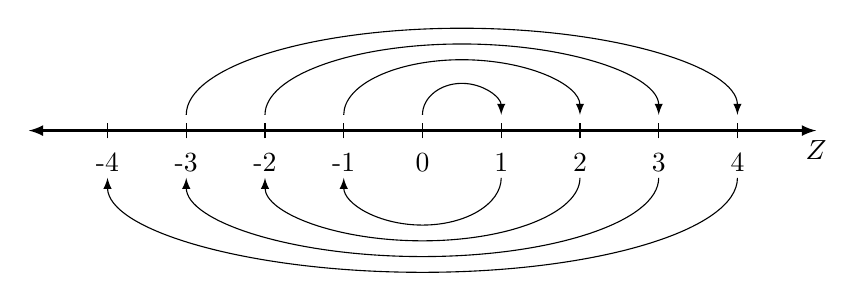
\begin{tikzpicture}[%
    >=latex
]
    \draw[<->, thick] (-5, 0) to (5, 0) node[below] {$\mathbb{Z}$};
    \foreach\x in {-4, -3, -2, -1, 0, 1, 2, 3, 4}{%
        \draw (\x, -0.1) to (\x, 0.1);
        \node at (\x, -0.4) {\x};
    }
    \draw[->] (0, 0.2) arc(180:0:0.5 and 0.4);
    \draw[->] (1, -0.6) arc(0:-180:1 and 0.6);
    \draw[->] (-1, 0.2) arc(180:0:1.5 and 0.7);
    \draw[->] (2, -0.6) arc(0:-180:2 and 0.8);
    \draw[->] (-2, 0.2) arc(180:0:2.5 and 0.9);
    \draw[->] (3, -0.6) arc(0:-180:3 and 1);
    \draw[->] (-3, 0.2) arc(180:0:3.5 and 1.1);
    \draw[->] (4, -0.6) arc(0:-180:4 and 1.2);
\end{tikzpicture}
            \caption{Diagram of a Bijection Between
                     $\mathbb{N}$ and $\mathbb{Z}$.}
            \label{fig:Bijection_N_and_Z}
        \end{figure}
        One of the standard results about countable sets is
        that their subsets are also countable. This theorem
        relies, in a very subtle way, the use of the axiom
        of choice. There are a few stepping stones to get
        there. We will accept the various
        Cantor-Schr\"{o}eder-Bernstein theorems, which say
        the following:
        \begin{ltheorem}
              {First Cantor-Schr\"{o}eder-Bernstein Theorem}
              {First_Cantor_Schroeder_Bernstein}
            If $A$ and $B$ are sets such that there is an injective
            function $f:A\rightarrow{B}$ and an injective function
            $g:B\rightarrow{A}$, then there is a bijective function
            $h:A\rightarrow{B}$.
        \end{ltheorem}
        \begin{ltheorem}
              {Second Cantor-Schr\"{o}eder-Bernstein Theorem}
              {Second_Cantor_Schroeder_Bernstein}
            If $A$ and $B$ are sets such that there is a surjective
            function $f:A\rightarrow{B}$ and a surjective function
            $g:B\rightarrow{A}$, then there is a bijective function
            $h:A\rightarrow{B}$.
        \end{ltheorem}
        \par\hfill\par
        Using cardinalities, this says that if
        $\mathrm{Card}(A)\leq\mathrm{Card}(B)$ and $\mathrm{Card}(B)\leq\mathrm{Card}(A)$, then
        $\mathrm{Card}(A)=\mathrm{Card}(B)$. With this notation it becomes more
        intuitive. We will use this to prove that various sets are
        countable. Many sets that appear to be larger than $\mathbb{N}$
        can shown to to be the same size as $\mathbb{N}$ by finding
        a simple injective function, without finding an explicit
        bijection.
        \begin{ltheorem}
              {Third Cantor-Schr\"{o}eder-Bernstein Theorem}
              {Third_Cantor_Schroeder_Bernstein}
            If $A$, $B$, and $C$ are sets such that
            $A\subseteq{B}\subseteq{C}$, and if $A$ and $C$ are equivalent
            sets, then $B$ and $C$ are equivalent sets.
        \end{ltheorem}
        \par\hfill\par
        This says that if $\mathrm{Card}(A)\leq\mathrm{Card}(B)\leq\mathrm{Card}(C)$,
        and if $\mathrm{Card}(A)=\mathrm{Card}(C)$, then $\mathrm{Card}(B)=\mathrm{Card}(C)$.
        \begin{theorem}
            \label{thm:Measure_Theory_NxN_Is_Countable}
            $\mathbb{N}\times\mathbb{N}$ is countably infinite.
        \end{theorem}
        \begin{proof}
            There is a trivial injection
            $f:\mathbb{N}\rightarrow\mathbb{N}\times\mathbb{N}$
            defined by:
            \begin{equation}
                f(n)=(n,0)
            \end{equation}
            There is also an injection
            $g:\mathbb{N}\times\mathbb{N}\rightarrow\mathbb{N}$
            defined by:
            \begin{equation}
                g(n.m)=2^{n}3^{m}
            \end{equation}
            Since 2 and 3 are co-prime, if
            $g(n_{1},m_{1})=g(n_{2},m_{2})$, then
            $(n_{1},m_{1})=(n_{2},m_{2})$. Thus, $g$ is an injection.
            By the Cantor-Schr\"{o}eder-Bernstein Theorem, there is a
            bijection $h:\mathbb{N}\rightarrow\mathbb{N}\times\mathbb{N}$.
        \end{proof}
        One can intuitively see that the set of all positive
        rational numbers $\mathbb{Q}^{+}$ is countable by examining
        the zig-zag pattern shown in
        Fig.~\ref{fig:Bijection_N_and_Q_Plus}.
        Thm.~\ref{thm:Measure_Theory_NxN_Is_Countable} also
        shows this in a more rigorous way that. We can create
        a one-to-one correspondence with
        $\mathbb{N}\times\mathbb{N}$ by mapping
        $pq^{\minus{1}}\mapsto(p,q)$. Thus $\mathbb{Q}^{+}$
        and $\mathbb{N}\times\mathbb{N}$ are equivalent sets.
        But $\mathbb{N}\times\mathbb{N}$ and $\mathbb{N}$
        are equivalent sets, and therefore $\mathbb{Q}^{+}$
        is countable.
        Thm.~\ref{thm:Measure_Theory_NxN_Is_Countable} can also be used
        to show that the countable union of countable sets is also
        countable.
        \begin{ltheorem}{Equivalence of Countable Sets}
              {Countable_iff_exists_inj_to_N}
            A set $A$ is countable if and only if there is an injective
            function $f:A\rightarrow\mathbb{N}$.
        \end{ltheorem}
        Thm.~\ref{thm:Countable_iff_exists_inj_to_N} seems
        intuitively obvious, the injective function is
        simply the listing function. For a finite set, this
        is precisely how one constructs such an injection.
        For an infinite set $A$, this is equivalent to
        showing that any infinite subset of $\mathbb{N}$ is
        equivalent to $\mathbb{N}$. The standard proof
        using \textit{induction}, but actually has the axiom
        of choice underlying it.
        \begin{theorem}
            If $\mathcal{A}$ is a countably infinite set
            such that, for all $A\in\mathcal{A}$, $A$ is
            a non-empty countable set, then the set:
            \begin{equation}
                S=\bigcup_{A\in\mathcal{A}}A
            \end{equation}
            Is a countable set.
        \end{theorem}
        \begin{proof}
            If $\mathcal{F}$ is finite, then we are done. Suppose not.
            Let $A:\mathbb{N}\rightarrow\mathcal{A}$ be a bijection,
            and define:
            \begin{equation}
                S=\bigcup_{n\in\mathbb{N}}A_{n}
            \end{equation}
            Also, let:
            \begin{equation}
                \mathcal{F}_{n}
                =\{f:A_{n}\rightarrow\mathbb{N}:
                    f\textrm{ is injective}\}
            \end{equation}
            Since, for all $n\in\mathbb{N}$, $A_{n}$ is
            non-empty and countable, $\mathcal{F}_{n}$
            is non-empty. Let:
            \begin{equation}
                \mathcal{F}
                =\bigcup_{n\in\mathbb{N}}\mathcal{F}_{n}
            \end{equation}
            Thus, by the axiom of choice, there is a function
            $F:\mathbb{N}\rightarrow\mathcal{F}$ such that, for all
            $n\in\mathbb{N}$, $F_{n}\in\mathcal{F}_{n}$. For
            $x\in{S}$, let:
            \begin{equation}
                \varphi_{x}
                =\inf\{n\in\mathbb{N}:x\in{A}_{n}\}
            \end{equation}
            By the well-ordering of $\mathbb{N}$, for all
            $x\in{S}$, $\varphi_{x}$ is well defined. Let
            $\phi:S\rightarrow\mathbb{N}\times\mathbb{N}$
            be defined by:
            \begin{equation}
                \phi(x)
                =\big(\varphi_{x},F_{\varphi_{x}}(x)\big)
            \end{equation}
            Then $\phi$ is an injection. For if
            $\big(\varphi_{x},F_{\varphi_{x}}(x)\big)=%
             \big(\varphi_{y},F_{\varphi_{x}}(y)\big)$, then
            $\varphi_{x}=\varphi_{y}$, and thus
            $F_{\varphi(x)}(x)=F_{\varphi(x)}(y)$. But
            $F_{\varphi_{x}}$ is an injection, and
            thus $x=y$. Therefore $\phi$ is an injection.
            But $\mathbb{N}\times\mathbb{N}$ and $\mathbb{N}$
            are equivalent sets, and thus there's an
            injection $f:\mathbb{N}\times\mathbb{N}$. And
            the composition of injective functions is again
            injective, and thus
            $\phi\circ{f}:S\rightarrow\mathbb{N}$ is an
            injective function. But by
            Thm.~\ref{thm:Countable_iff_exists_inj_to_N},
            if there is an injective function
            $f:S\rightarrow\mathbb{N}$, then $S$ is
            countable. Therefore, etc.
        \end{proof}
        \begin{theorem}
            If $X$ is infinite, then there exists a
            countably infinite set $A\subseteq{X}$.
        \end{theorem}
        \begin{proof}
            If $A$ is finite, then we are done. Suppose not.
            For $n\in\mathbb{N}$, let:
            \begin{equation}
                A_{n}
                =\{g:\mathbb{Z}_{n}\rightarrow{A}:f\textrm{ is inective}\}
            \end{equation}
            Also, define:
            \begin{equation}
                \mathcal{F}=\bigcup_{n\in\mathbb{N}}A_{n}
            \end{equation}
            But by the axiom of choice, there is a function
            $f:\mathbb{N}\rightarrow\mathcal{F}$ such that
            $f_{n}\in{A}_{n}$. But then, for all
            $n\in\mathbb{N}$, the range of $f_{n}$ is finite.
            \begin{equation}
                A=\bigcup_{n\in\mathbb{N}}f_{n}
                    \Big(\mathbb{Z}_{n}\Big)
            \end{equation}
            Then $A\subseteq{X}$ is countably infinite.
        \end{proof}
        The set of rational numbers, $\mathbb{Q}$, is also
        countable. We may intuitively think of $\mathbb{N}$
        as being smaller than $\mathbb{Q}$, since there are
        simple \textit{surjections} that can be constructed
        from $\mathbb{Q}$ to $\mathbb{N}$. There is also a
        surjection from $\mathbb{N}$ onto $\mathbb{Q}^{+}$,
        as is shown in Fig.~\ref{fig:Bijection_N_and_Q_Plus}.
        To construct such a surjection, write out all of the
        positive rational numbers in a grid so that $a_{nm}$
        is the number $n/m$. Then zig-zag along the diagonals
        to construct the function. Thus there is a surjection
        $f:\mathbb{Q}^{+}\rightarrow\mathbb{N}$
        and a surjection
        $g:\mathbb{N}\rightarrow\mathbb{Q}^{+}$.
        \begin{figure}[H]
            \centering
            \captionsetup{type=figure}
            \resizebox{0.7\textwidth}{!}{%
                %--------------------------------Dependencies----------------------------------%
%   tikz                                                                       %
%       arrows.meta                                                            %
%-------------------------------Main Document----------------------------------%
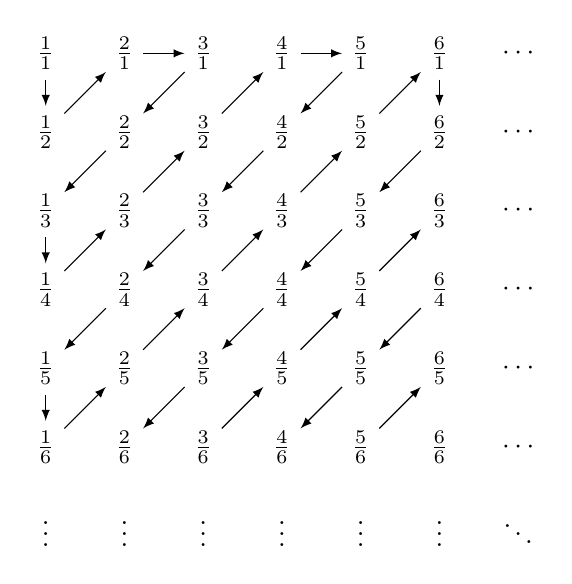
\begin{tikzpicture}[%
    >=latex
]
    \foreach\y in {1, 2, 3, 4, 5, 6}{%
        \foreach\x in {1, 2, 3, 4, 5, 6}{%
            \node (\x\y) at (\x, 7-\y) {$\frac{\x}{\y}$};
        }
    }
    \foreach\x in {1, 2, 3, 4, 5, 6}{%
        \node at (7, \x) {$\cdots$};
        \node at (\x, 0) {$\vdots$};
    }
    \node at (7, 0) {$\ddots$};
    \draw[->] (11) to (12);
    \draw[->] (12) to (21);
    \draw[->] (21) to (31);
    \draw[->] (31) to (22);
    \draw[->] (22) to (13);
    \draw[->] (13) to (14);
    \draw[->] (14) to (23);
    \draw[->] (23) to (32);
    \draw[->] (32) to (41);
    \draw[->] (41) to (51);
    \draw[->] (51) to (42);
    \draw[->] (42) to (33);
    \draw[->] (33) to (24);
    \draw[->] (24) to (15);
    \draw[->] (15) to (16);
    \draw[->] (16) to (25);
    \draw[->] (25) to (34);
    \draw[->] (34) to (43);
    \draw[->] (43) to (52);
    \draw[->] (52) to (61);
    \draw[->] (61) to (62);
    \draw[->] (62) to (53);
    \draw[->] (53) to (44);
    \draw[->] (44) to (35);
    \draw[->] (35) to (26);
    \draw[->] (36) to (45);
    \draw[->] (45) to (54);
    \draw[->] (54) to (63);
    \draw[->] (64) to (55);
    \draw[->] (55) to (46);
    \draw[->] (56) to (65);
\end{tikzpicture}
            }
            \caption{Diagram of a Surjection from
                     $\mathbb{N}$ onto $\mathbb{Q}^{+}$.}
            \label{fig:Bijection_N_and_Q_Plus}
        \end{figure}
        We can modify Fig.~\ref{fig:Bijection_N_and_Q_Plus}
        slightly to create a surjection between $\mathbb{N}$
        and $\mathbb{Q}$, see
        Fig.~\ref{fig:Bijection_N_and_Q}.
        It is important to note that this bijection will not
        preserve the order of the rational numbers. The
        bijection will have to jump around back and forth.
        Any such bijection will be forced to do this, as the
        rationals are everywhere dense on $\mathbb{R}$. Any
        monotonic sequence of $\mathbb{Q}$ cannot possibly
        be a bijection.
        \begin{theorem}
            If $A$ is a countably infinite set and
            $B\subseteq{A}$, then $B$ is countable.
        \end{theorem}
        \begin{proof}
            As $A$ is countably infinite, there is a bijection
            $a:\mathbb{N}\rightarrow{A}$. Define:
            \begin{equation}
                K=\{n\in\mathbb{N}:a_{n}\in{B}\}
            \end{equation}
            As $B\subseteq{A}$,
            this set contains a subsequence of points in
            $\mathbb{N}$ that get mapped into $B$. If $K$ is finite,
            then $B$ is finite, and if not then $K$ is countably
            infinite, and thus $B$ is countably infinite.
        \end{proof}
        \begin{figure}[H]
            \centering
            \captionsetup{type=figure}
            \resizebox{\textwidth}{!}{%
                %--------------------------------Dependencies----------------------------------%
%   amsmath                                                                    %
%   tikz                                                                       %
%       arrows.meta                                                            %
%-------------------------------Main Document----------------------------------%
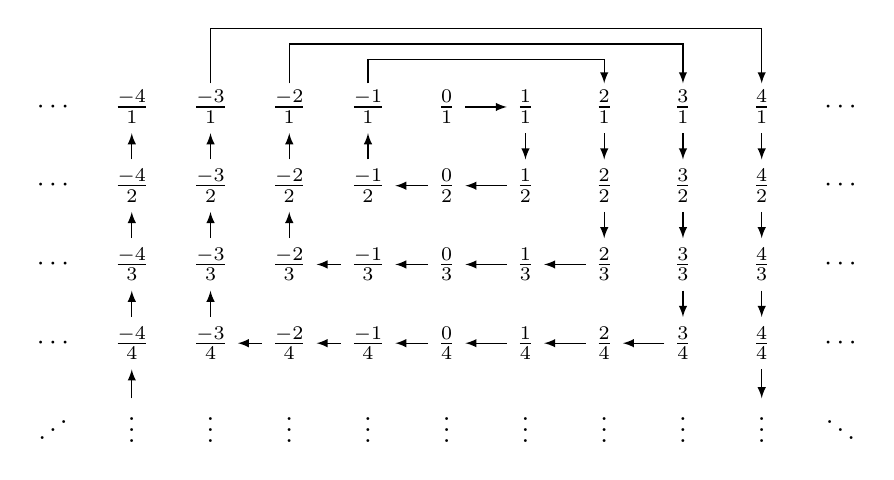
\begin{tikzpicture}[%
    >=latex
]
    \foreach\y in {1, 2, 3, 4}{%
        \foreach\x in {-4, -3, -2, -1, 0, 1, 2, 3, 4}{%
            \node (\x\y) at (\x, 7-\y) {$\frac{\x}{\y}$};
        }
    }
    \foreach\x in {-4, -3, -2, -1, 0, 1, 2, 3, 4}{%
        \node at (\x, 2) {$\vdots$};
    }
    \foreach\y in {3, 4, 5, 6}{%
        \node at (5, \y) {$\cdots$};
        \node at (-5, \y) {$\cdots$};
    }
    \node at (5, 2) {$\ddots$};
    \node at (-5, 2) {$\reflectbox{\ensuremath{\ddots}}$};
    \draw[->] (01) to (11);
    \draw[->] (11) to (12);
    \draw[->] (12) to (02);
    \draw[->] (02) to (-12);
    \draw[->] (-12) to (-11);
    \draw[->] (-1, 6.3) to (-1, 6.6)
                        to (2, 6.6)
                        to (2, 6.3);
    \draw[->] (21) to (22);
    \draw[->] (22) to (23);
    \draw[->] (23) to (13);
    \draw[->] (13) to (03);
    \draw[->] (03) to (-13);
    \draw[->] (-13) to (-23);
    \draw[->] (-23) to (-22);
    \draw[->] (-22) to (-21);
    \draw[->] (-2, 6.3) to (-2, 6.8)
                        to (3, 6.8)
                        to (3, 6.3);
    \draw[->] (31) to (32);
    \draw[->] (32) to (33);
    \draw[->] (33) to (34);
    \draw[->] (34) to (24);
    \draw[->] (24) to (14);
    \draw[->] (14) to (04);
    \draw[->] (04) to (-14);
    \draw[->] (-14) to (-24);
    \draw[->] (-24) to (-34);
    \draw[->] (-34) to (-33);
    \draw[->] (-33) to (-32);
    \draw[->] (-32) to (-31);
    \draw[->] (-3, 6.3) to (-3, 7)
                        to (4, 7)
                        to (4, 6.3);
    \draw[->] (41) to (42);
    \draw[->] (42) to (43);
    \draw[->] (43) to (44);
    \draw[->] (44) to (4, 2.3);
    \draw[->] (-4, 2.3) to (-44);
    \draw[->] (-44) to (-43);
    \draw[->] (-43) to (-42);
    \draw[->] (-42) to (-41);
\end{tikzpicture}
            }
            \caption{Diagram of a Surjection from
                     $\mathbb{N}$ onto $\mathbb{Q}$.}
            \label{fig:Bijection_N_and_Q}
        \end{figure}
        \begin{theorem}
            If $A$ is an infinite set, then there exists a
            countable subset $B\subseteq{A}$.
        \end{theorem}
        \begin{proof}
            If $A$ is infinite then there is an
            $a_{1}\in{A}$. But, as $A$ is infinite,
            $A\setminus\{a_{1}\}$ is infinite, and there
            is an $a_{2}\in{A}\setminus\{a_{1}\}$. Continuing
            we obtain a sequence of distinct elements in $A$.
            Let $B=\{a_{n}:n\in\mathbb{N}\}$. Then
            $B\subseteq{A}$, and $B$ is countable.
        \end{proof}
        \begin{lexample}{}{Disjoint_Union_of_Intervals_is_Countable}
            Suppose we have a collection of disjoint intervals
            of $\mathbb{R}$. This collection is either finite
            or countable. For in every interval, choose a
            rational number $q_{n}$. Let
            $A=\{q_{1},q_{2},\hdots\}$. Then
            $A\subseteq\mathbb{Q}$, and thus $A$ is either
            finite or countable. But this is also an enumeration
            of the intervals in the collection, and thus the
            collection is either finite or countable.
        \end{lexample}
        Given a countable collection of sets
        $A=\{\mathcal{A}_{1},\mathcal{A}_{2},\hdots\}$ such
        that, for all $n\in\mathbb{N}$, $\mathcal{A}_{n}$ is
        also a countable set, then the union is countable. That is:
        \begin{equation}
            B=\bigcup_{n=1}^{\infty}\mathcal{A}_{n}
        \end{equation}
        is a countable set. The proof of this is a mimicry of
        the proof of the countability of $\mathbb{Q}$. Not
        every set is either finite or countable. The real numbers,
        $\mathbb{R}$, is an example of an \textit{uncountable}
        set. First, some notes on the power set of a set.
        \begin{lexample}{}{Basic_Power_Set}
            \begin{subequations}
                If $\Omega=\{1,2\}$, then the power set is:
                \begin{equation}
                    \mathcal{P}(\Omega)=
                    \big\{\emptyset,\{1\},\{2\},\{1,2\}\big\}
                \end{equation}
                We must consider the empty set, since for any set
                $A$, $\emptyset\subseteq{A}$. As another example,
                let $\Omega=\{1,2,3\}$. Then:
                \begin{equation}
                    \mathcal{P}(\Omega)=
                    \big\{\emptyset,\{1\},\{2\},\{3\},\{1,2\},
                      \{1,3\},\{2,3\},\{1,2,3\}\big\}
                \end{equation}
                We see that, in the first example, a set with
                2 elements has a power set with 4 elements. In the
                second example we see that a set with 3 elements has
                a power set with 8 elements. This pattern continues
                for finite sets. If $A$ has $n$ elements, then
                $\mathcal{P}(A)$ has $2^{n}$ elements. If
                $A$ is an infinite set, then $\mathcal{P}(A)$ is
                uncountable. Indeed:
                \begin{equation}
                    \mathrm{Card}\big(\mathcal{P}(\mathbb{N})\big)=
                    \mathrm{Card}(\mathbb{R})
                \end{equation}
                We can show this by using the binary representation
                of real numbers. We construct a bijection as
                follows: If $A\subseteq\mathbb{N}$, then
                let $r_{A}=0.n_{1}n_{2}\hdots$ where:
                \begin{equation}
                    n_{i}=
                    \begin{cases}
                        0,&i\notin{A}\\
                        1,&i\in{A}
                    \end{cases}
                \end{equation}
                The function
                $f:\mathcal{P}(\mathbb{N})\rightarrow[0,1]$
                defined by $f(A)=r_{A}$ is thus a bijection.
                That is, every element of $[0,1]$ gets mapped to in
                a one-to-one manner. The potentially tricky numbers are
                0 and 1, but $f(\emptyset)=0$, and $f(\mathbb{N})=1$.
                Thus $\mathcal{P}(\mathbb{N})$ and $[0,1]$ are of the
                same cardinality. But $(0,1)$ and $\mathbb{R}$
                are of the same cardinality. To see this, consider
                the graph of the function
                $g:(0,1)\rightarrow\mathbb{R}$ defined as:
                \begin{equation}
                    g(x)=\frac{2x-1}{x(1-x)}
                \end{equation}
                This is a bijection between the unit interval
                $(0,1)$ and $\mathbb{R}$. One can also use the
                \textit{stereographic projection} to show this.
                But also $[0,1]$ and $(0,1)$ have the same cardinality.
                For this, consider the following function:
                \begin{equation}
                    f(x)=
                    \begin{cases}
                        \frac{1}{2},&x=0\\
                        \frac{1}{2^{n+2}},&x=\frac{1}{2^{n}}\\
                        x,&\textrm{Otherwise}
                    \end{cases}
                \end{equation}
                A graph of this is shown in
                Fig.~\ref{fig:Measure_Theory_Bijection_Closed_I_to_Open}.
                Therefore, $\mathbb{R}$ and
                $\mathcal{P}(\mathbb{N})$ have the same cardinality.
                This can then be used to show that $\mathbb{R}$ is
                uncountable.
            \end{subequations}
        \end{lexample}
        \begin{figure}[H]
            \centering
            \captionsetup{type=figure}
            \documentclass[crop,class=article]{standalone}
%----------------------------Preamble-------------------------------%
\usepackage{tikz}                       % Drawing/graphing tools.
\usetikzlibrary{arrows.meta}            % Latex and Stealth arrows.
%--------------------------Main Document----------------------------%
\begin{document}
    \begin{tikzpicture}[>=Latex, scale=2]
        \draw[->] (-0.15in, 0) to (1.1in, 0) node[above] {$x$};
        \draw[->] (0, -0.15in) to (0, 1.1in) node[right] {$y$};
        \draw (0, 0) to (1in, 1in);
        \draw[fill=black, draw=black] (0, 0.5in) circle (0.3mm);
        \foreach\x in{1in, 0.5in, 0.25in, 0.125in, 0.0625in, 0.03125in}{
            \draw[fill=white, draw=black] (\x, \x) circle (0.3mm);
            \draw[fill=black, draw=black] (\x, 0.25*\x) circle (0.3mm);
        }
    \end{tikzpicture}
\end{document}
            \caption{Bijection from $[0,1]$ to $(0,1)$.}
            \label{fig:Measure_Theory_Bijection_Closed_I_to_Open}
        \end{figure}
        The power set of any set is strictly larger than the
        original set. If $\Omega$ is finite with $n$ elements, it
        can be shown that $\mathcal{P}(\Omega)$ has $2^{n}$
        elements. For infinite sets, there is a trivial surjection
        from $\mathcal{P}(\Omega)$ onto $\Omega$: for any element
        $x$, let $f(\{x\})=x$. This shows that
        $\mathrm{Card}(\Omega)\leq\mathrm{Card}(\mathcal{P}(\Omega))$. We now show
        that the inequality is strict.
        \begin{theorem}
            If $\Omega$ is a set, then there is no bijection
            $f:\Omega\rightarrow\mathcal{P}(\Omega)$
        \end{theorem}
        \begin{proof}
            For suppose not, and let
            $f:\Omega\rightarrow\mathcal{P}(\Omega)$ be such a
            bijection. Define:
            \begin{equation}
                A=\{x\in\Omega:x\in{f}(x)\}
            \end{equation}
            Then $A\subseteq\Omega$, and thus
            $A\in\mathcal{P}(\Omega)$. But then the complement of
            $A$ is also an element of $\mathcal{P}(\Omega)$. But
            $f$ is a bijection and thus there is an $x\in\Omega$
            such that $f(x)=A^{C}$. If $x\in{f}(x)$, then
            $x\in{A}$, a contradiction as $f(x)=A^{C}$, and thus
            $x\in{A}^{C}$ as well. Therefore $x\notin{f}(x)$. But
            then $x\in{A}^{C}$. But, from the definition of $A$,
            since $x\in{A}^{C}$ and $f(x)=A^{C}$, $x\in{f}(x)$
            and thus $x\in{A}$, a contradiction. Thus there is no
            $x$ such that $f(x)=A^{C}$. Therefore, $f$ is not a
            bijection.
        \end{proof}
        From this we conclude that $\mathcal{P}(\mathbb{N})$
        is an uncountable infinite set. But since $\mathbb{R}$
        and $\mathcal{P}(\mathbb{N})$ have the same cardinality,
        $\mathbb{R}$ is also uncountable.
        If a set $A$ has the same cardinality as $\mathbb{R}$,
        we say that $A$ has the cardinality of the continuum.
        \begin{lexample}{}{Bijection_from_closed_to_open_interval}
            There is a bijection between the open unit
            square $(0,1)\times(0,1)$ and the open unit interval
            $(0,1)$. For an element $(x,y)\in(0,1)\times(0,1)$,
            let $z\in(0,1)$ be defined as
            $z=0.x_{1}y_{1}x_{2}y_{2}x_{3}y_{3}\dots$ This is
            a bijection, for all $(x,y)$ in the square there is
            a corresponding $z\in(0,1)$, and for all
            $z\in(0,1)$ there is a corresponding element of
            $(0,1)\times(0,1)$. We can say that $(x,y)$ can
            be coded into $z$, and $z$ can be decoded into
            $(x,y)$. Hence, $(0,1)\times(0,1)$ has the cardinality
            of the continuum. By stereographic projection and induction
            we obtain:
            \par\hfill\par
            \begin{subequations}
                \begin{minipage}[b]{0.49\textwidth}
                    \centering
                    \begin{equation}
                        \mathrm{Card}(\mathbb{R}^{2})=\mathrm{Card}(\mathbb{R})
                    \end{equation}
                \end{minipage}
                \hfill
                \begin{minipage}[b]{0.49\textwidth}
                    \centering
                    \begin{equation}
                        \mathrm{Card}(\mathbb{R}^{n})=\mathrm{Card}(\mathbb{R})
                    \end{equation}
                \end{minipage}
                \par
            \end{subequations}
        \end{lexample}
        \begin{lexample}{}{Space_of_Sequences}
            Consider the set of all real-valued sequences. We've seen
            that any real number can be represented as a function
            $f:\mathbb{N}\rightarrow\{0,1\}$. A real-valued sequence
            is a function $a:\mathbb{N}\rightarrow\mathbb{R}$, and
            thus the set of real-valued sequences can be seen as the
            set of functions whose domain is $\mathbb{N}$ and whose
            range is the set of all functions
            $f:\mathbb{N}\rightarrow\{0,1\}$. So given a sequence
            $a$, the image of $a_{n}$, for $n\in\mathbb{N}$, is a
            function $f_{n}:\mathbb{N}\rightarrow\{0,1\}$. Therefore
            the set of all real-valued sequences can be represented
            as the set of all functions
            $g:\mathbb{N}\times\mathbb{N}\rightarrow\{0,1\}$, where
            $g(n,m)=f_{n}(m)$. But $\mathbb{N}\times\mathbb{N}$ is
            countable, and thus the set of all functions of the form
            $g:\mathbb{N}\times\mathbb{N}\rightarrow\{0,1\}$ has the
            same cardinality as the set of all functions of the form
            $f:\mathbb{N}\rightarrow\{0,1\}$. But this has the
            cardinality of the continuum. Therefore, the set of all
            real-valued sequences has the cardinality of the continuum.
        \end{lexample}

    \chapter{Order Theory}
        \section{Order Theory}
    \subsection{Relations}
        \begin{ldefinition}{Relation on a Set}{Relation}
            A relation on a set $A$ is a subset $R$ of
            $A\times{A}$. That is, $R\subseteq{A}\times{A}$.
            For elements $(a,b)\in{R}$ we write $aRb$.
        \end{ldefinition}
        For a relation $R$ it is not necessary true that $aRb$
        implies $bRa$, nor is it necessarily true that $aRa$. These
        are called symmetric and reflexive relations, respectively.
        There are many basic properties that relations have, and we
        prove them now.
        \begin{theorem}
            \label{thm:Cartesian_Product_Is_Relation}%
            If $A$ is a set, then $A\times{A}$ is a relation on $A$.
        \end{theorem}
        \begin{proof}
            For if $A$ is a set, then
            $A\times{A}\subseteq{A}\times{A}$. Therefore, etc.
        \end{proof}
        \begin{theorem}
            \label{thm:Empty_Set_Is_Relation}%
            If $A$ is a set, and then $\emptyset$ is a relation
            on $A$.
        \end{theorem}
        \begin{proof}
            For if $A$ is a set, then
            $\emptyset\subseteq{A}\times{A}$. Therefore, etc.
        \end{proof}
        These provide the two most basic examples of relations on a
        set. The empty set is the relation that says no two elements
        are related. Indeed, even single elements are unrelated to
        themselves. The second, the entire Cartesian product
        $A\times{A}$, says that everything is related. These are the
        two extreme cases, but provide useful examples and
        counterexamples in various contexts. More useful is that the
        union and intersection of relations is also a relation. We
        prove this now.
        \begin{theorem}
            \label{thm:Intersection_of_Relations_Is_Relation}%
            If $A$ is a set and if $R_{1}$ and $R_{2}$ are relations
            on $A$, then $R_{1}\cap{R}_{2}$ is a relation on $A$.
        \end{theorem}
        \begin{proof}
            For let $R=R_{1}\cap{R}_{2}$ and suppose $R$ is not a
            relation on $A$. Then there is an $x\in{R}$ such that
            $x\notin{A}\times{A}$. But if $x\in{R}$ then
            $x\in{R}_{1}$ and $x\in{R}_{2}$. But for all
            $x\in{R}_{1}$, $x\in{A}\times{A}$, since $R_{1}$ is a
            relation on $A$, a contradiction as
            $x\notin{A}\times{A}$. Therefore, $R$ is a relation on
            $A$.
        \end{proof}
        \begin{theorem}
            \label{thm:Set_Theory_Union_of_Relations_Is_Relation}
            If $A$ is a set and if $R_{1}$ and $R_{2}$ are relations
            on $A$, then $R_{1}\cup{R}_{2}$ is a relation on $A$.
        \end{theorem}
        \begin{proof}
            For let $R=R_{1}\cup{R}_{2}$ and suppose $R$ is not a
            relation on $A$. Then there is an $x\in{R}$ such that
            $x\notin{A}\times{A}$. But if $x\in{R}$ then
            $x\in{R}_{1}$ or $x\in{R}_{2}$. But for all $x\in{R}_{1}$
            and for all $x\in{R}_{2}$,
            $x\in{A}\times{A}$, since $R_{1}$ and $R_{2}$ are
            relations on $A$, a contradiction. Therefore, etc.
        \end{proof}
        \begin{theorem}
            If $A$ is a set and $R$ is a relation on $A$, then there
            is a relation $\mathcal{U}$ on $A$ such that
            $R\cap\mathcal{U}=R$.
        \end{theorem}
        \begin{proof}
            For let $\mathcal{U}={A}\times{A}$. Then by
            Thm.~\ref{thm:Cartesian_Product_Is_Relation},
            $A\times{A}$ is a relation on $A$. But since $R$ is
            a relation, $R\subseteq{A}\times{A}$. But then
            $R\cap\mathcal{U}=R$. Therefore, etc.
        \end{proof}
        \begin{theorem}
            If $A$ is a set and $R$ is a relation on $A$, then there
            is a relation $\mathcal{U}$ on $A$ such that
            $R\cup\mathcal{U}=R$
        \end{theorem}
        \begin{proof}
            For let $\mathcal{U}=\emptyset$. Then by
            Thm.~\ref{thm:Empty_Set_Is_Relation},
            $\mathcal{U}$ is a relation. But if $R$ is a set, then
            $R\cup\emptyset=R$. Thus, $R\cup\mathcal{U}=R$.
            Therefore, etc.
        \end{proof}
        Since a general relation is simply a subset of $A\times{A}$,
        there's not much structure on them, and thus there's not a lot
        that can be said about them. We can add more constraints to
        certain relations to get the more familiar properties
        we're used to.
        \begin{ldefinition}{Reflexive Relations}
                           {Reflexive_Relations}
            A reflexive relation on a set $A$ is a
            relation $R$ on $A$ such that for all $a\in{A}$
            it is true that $aRa$.
        \end{ldefinition}
        A reflexive relation on $A$ is simply any subset of
        $A\times{A}$ that contains the entire \textit{diagonal}. That,
        all of the pairs $(a,a)$. A reflexive relation can contain more
        than this, however. The only strict requirement is that
        $aRa$ for all $a\in{A}$.
        \begin{theorem}
            If $A$ is a set, and if $R_{1}$ and $R_{2}$ are reflexive
            relations on $A$, then $R_{1}\cap{R}_{2}$ is a reflexive
            relation on $A$.
        \end{theorem}
        \begin{proof}
            For let $R=R_{1}\cap{R}_{2}$. Then by
            Thm.~\ref{thm:Intersection_of_Relations_Is_Relation},
            $R$ is a relation. Suppose $R$ is not reflexive.
            Then there is an $a\in{A}$ such that $(a,a)\notin{R}$.
            But if $a\in{A}$, then $(a,a)\in{R}_{1}$, since $R_{1}$
            is reflexive. Similarly, $(a,a)\in{R}_{2}$ since
            $R_{2}$ is reflexive. But if $(a,a)\in{R}_{1}$ and
            $(a,a)\in{R}_{2}$, then $(a,a)\in{R}$ since
            $R=R_{1}\cap{R}_{2}$, a contradiction. Therefore,
            $R$ is reflexive.
        \end{proof}
        \begin{theorem}
            If $A$ is a set, if $R_{1}$ is a reflexive relation on
            $A$, and if $R_{2}$ is a relation on $A$, then
            $R_{1}\cup{R}_{2}$ is a reflexive relation on $A$.
        \end{theorem}
        \begin{proof}
            For let $R=R_{1}\cup{R}_{2}$. Since $R_{1}$ and $R_{2}$ are
            relations, by
            Thm.~\ref{thm:Set_Theory_Union_of_Relations_Is_Relation},
            $R$ is a relation. Suppose it is not reflexive.
            Then there is an $a\in{A}$ such that
            $(a,a)\notin{R}$. But if $a\in{A}$ then $(a,a)\in{R}_{1}$
            since $R_{1}$ is reflexive. But if $(a,a)\in{R}_{1}$ then
            $(a,a)\in{R}_{1}\cup{R}_{2}$, a contradiction.
            Therefore, etc.
        \end{proof}
        Given an arbitrary relation $R$ on a set $A$, it may not be
        true that $R$ is reflexive. It may often be useful to add in
        only the necessary points of $A$ that will make $R$
        reflexive. This is called the reflexive closure of $R$.
        \begin{ldefinition}{Reflexive Closure of a Relation}
                           {Reflexive_Closure_of_Relation}
            The reflexive closure of a relation $R$ on a set $A$
            is the set:
            \begin{equation}
                S=R\cup\{(a,a):a\in{A}\}
            \end{equation}
        \end{ldefinition}
        \begin{theorem}
            If $A$ is a set, $R$ is a relation on $A$, and if $S$ is the
            reflexive closure of $R$, then $S$ is a reflexive relation on $A$.
        \end{theorem}
        \begin{theorem}
            \label{thm:Set_Theory_Refl_Clos_Is_Smallest_Refl_With_R}
            If $A$ is a set, if $R$ is a relation on $A$, if
            $S$ is the reflexive closure of $R$, and if $T$ is a
            reflexive relation on $A$ such that $R\subseteq{T}$, then
            $S\subseteq{T}$.
        \end{theorem}
        \begin{proof}
            For if $x\in{S}$, then either $x\in{R}$ or there is an
            $a\in{A}$ such that $x=(a,a)$. But if $x\in{R}$, then
            $x\in{T}$ since $R\subseteq{T}$. If $x\notin{R}$ then
            there is an $a\in{A}$ such that $x=(a,a)$. But $T$ is
            reflexive, and therefore $(a,a)\in{T}$. But then
            $x\in{T}$. Therefore, $S\subseteq{T}$.
        \end{proof}
        Thm.~\ref{thm:Set_Theory_Refl_Clos_Is_Smallest_Refl_With_R}
        says that the reflexive closure of a relation $R$ is, in a sense,
        the \textit{smallest} relation that is reflexive and contains
        $R$ as a subset.
        \begin{theorem}
            If $A$ is a set, $R_{1}$ and $R_{2}$ are relations on $A$,
            and if $S_{1}$ and $S_{2}$ are the reflexive closures of
            $R_{1}$ and $R_{2}$, respectively, then the reflexive closure
            of $R_{1}\cap{R}_{2}$ is:
            \begin{equation}
                S=S_{1}\cap{S}_{2}
            \end{equation}
        \end{theorem}
        \begin{proof}
            By the definition of reflexive closure, we have:
            \begin{align}
                S_{1}&=R_{1}\cup\{(a,a):a\in{A}\}
                \tag{Def.~\ref{def:Reflexive_Closure_of_Relation}}\\
                S_{1}&=R_{2}\cup\{(a,a):a\in{A}\}
                \tag{Def.~\ref{def:Reflexive_Closure_of_Relation}}\\
                \nonumber
                S_{1}\cap{S}_{2}&=
                (R_{1}\cup\{(a,a):a\in{A}\})
                \cap(R_{2}\cup\{(a,a):a\in{A}\})\\
                &=(R_{1}\cap{R}_{2})
                \cup\{(a,a):a\in{A}\}
                \tag{Distributive Law}
            \end{align}
            But by the definition of the transitive closure of
            $R_{1}\cap{R}_{2}$:
            \begin{equation}
                S=(R_{1}\cap{R}_{2})\cup\{(a,a):a\in{A}\}
                \tag{Def.~\ref{def:Reflexive_Closure_of_Relation}}
            \end{equation}
            Therefore, etc.
        \end{proof}
        \begin{ldefinition}{Symmetric Relations}
                           {Symmetric_Relations}
            A symmetric relation on a set $A$ is a
            relation $R$ on $A$ such that for all $a,b\in{A}$
            such that $aRb$, it is true that $bRa$.
        \end{ldefinition}
        \begin{ldefinition}{Transitive Relations}
                           {Transitive_Relations}
            A transitive relation on a set $A$ is a relation $R$ on $A$
            such that for all $a,b,c\in{A}$ such that $aRb$ and $bRc$,
            is it true that $aRc$.
        \end{ldefinition}
        \begin{ldefinition}{Transitive Closure}{Transitive_Closure}
            The transitive closure of a relation $R$ on a set
            $A$ is the the set $R^{t}\subseteq{A}\times{A}$ defined by:
            \begin{equation}
                R^{t}
            \end{equation}
        \end{ldefinition}
        \begin{ldefinition}{Asymmetric Relation}
                           {Asymmetric_Relation}
            An asymmetric relation on a set $A$ is a relation $R$
            on $A$ such that for all $a,b\in{A}$ such that $aRb$
            it is true that $(b,a)\notin{R}$.
        \end{ldefinition}
        \begin{ldefinition}{Total Relation}{Total_Relation}
            A total relation on a set $A$ is a relation $R$ on $A$ such
            that for all $a,b\in{A}$ it is true that either
            $aRb$ or $bRa$, or both.
        \end{ldefinition}
        The notion of equality can be defined as a relation
        with the following properties:
        \begin{enumerate}
            \item Equality is Reflexive: $a=a$ for all $a\in{A}$.
            \item Equality is Symmetric: $a=b$ if and only if $b=a$.
            \item Equality is Transitive: If $a=b$ and $b=c$, then $a=c$.
            \item The relation is uniquely defined by the set
                  $\{(a,a)\in A\times A:a\in A\}$.
        \end{enumerate}
        That is, equality can be seen as the \textit{diagonal} in the
        Cartesian product $A\times{A}$.
        \begin{ldefinition}{Antisymmetric Relation}
                           {Antisymmetric_Relation}
            An antisymmetric relation on a set $A$ is a relation $R$ on $A$
            such that for all $a,b\in{A}$ such that $aRb$ and $bRa$, it
            is true that $a=b$.
        \end{ldefinition}
    \subsection{Zorn's Lemma}
        A relation on a set $X$ is a subset
        $R\subseteq{X}\times{X}$. Given an element
        $(x,y)\in{R}$, we often write $xRy$ to denote this.
        Here we'll write $x\leq{y}$.
        \begin{ldefinition}{Ordered Sets}
              {Funct_Analysis_Ordered_Set}
            An ordered set is a set $X$ and a relation
            $\leq$ on $X$, denoted $(X,\leq)$ such that
            the following are true:
            \begin{enumerate}
                \item For all $x\in{X}$, $x\leq{x}$.
                \item For all $x,y\in{X}$ such that $x\leq{y}$ and
                      $y\leq{x}$, it is true that $x=y$.
                \item For all $x,y,z\in{X}$ such that $x\leq{y}$
                      and $y\leq{z}$, it is true that $x\leq{z}$.
            \end{enumerate}
        \end{ldefinition}
        \begin{ldefinition}{Majorants in Ordered Sets}{Majorant_in_Ord_Set}
            A majorant of a subset $Y\subseteq{X}$ of
            and ordered set $(X,\leq)$ is an element $x\in{X}$
            such that, for all $y\in{Y}$, it is true that
            $y\leq{x}$.
        \end{ldefinition}
        \begin{lexample}{}{Reverse_Containment_Example}
            Let $(X,d)$ be a metric space, and let
            $x_{0}\in{X}$. Define the following:
            \begin{equation}
                \mathscr{N}(x_{0})=
                \big\{\mathcal{V}\subseteq{X}:\mathcal{V}
                    \textrm{ is a neighborhood of $x_{0}$}\big\}
            \end{equation}
            We can order $\mathscr{N}$ by reverse containment.
            That is, We have the following relation:
            \begin{equation}
                \leq=\big\{(\mathcal{U},\mathcal{V})\in
                    \mathscr{N}(x_{0})\times\mathscr{N}(x_{0})
                    :\mathcal{V}\subseteq\mathcal{U}\big\}
            \end{equation}
            That is, we write $\mathcal{U}\leq\mathcal{V}$ if
            $\mathcal{V}$ is a subset of $\mathcal{U}$. Note
            that, for all $x_{0}$,
            $\mathscr{x_{0}}$ has a least element, or a minorant,
            but $X$ is such an element. But, if $\{x_{0}\}$ is
            not open, then there is no majorant.
        \end{lexample}
        \begin{ldefinition}{Totally Ordered Sets}
              {Funct_Analysis_Tot_Ord_Set}
            A totally ordered set is an ordered set
            $(X,\leq)$ such that, for all $x,y\in{X}$, either
            $x\leq{y}$ or $y\leq{x}$.
        \end{ldefinition}
        \begin{ldefinition}{Maximal Element}
              {Funct_Analysis_Maximal_Element}
            A maximal element of a subset $Y\subseteq{X}$ of
            a totally ordered set $(X,\leq)$ is an element $y$
            such that:
            \begin{equation}
                \{y'\in{Y}:y\leq{y}'\}=\{y\}
            \end{equation}
            Note that $y$ is not necessary a majorant for $Y$
            nor is $y$ necessarily unique.
        \end{ldefinition}
        \begin{ldefinition}{Inductively Ordered Sets}
              {Funct_Analysis_Induct_Ordered_Set}
            An inductively ordered set is an ordered set
            $)X,\leq)$ such that, for all totally ordered
            subsets $S\subseteq{X}$, there is a majorant
            $x\in{X}$ of $S$.
        \end{ldefinition}
        That is, there exists $x\in{X}$ such that, for all
        $y\in{S}$, $y\leq{x}$.
        \begin{lexample}{}{Trivial_Inductively_Ordered_Set}
            Let $X=\mathbb{R}$ and consider the set
            $\mathscr{N}(0)$. Then $\mathscr{N}(0)$ is
            not inductively ordered.
        \end{lexample}
        \begin{ltheorem}{Zorn's Lemma}{Zorns_Lemma}
            If $(X,\leq)$ is an inductively ordered set,
            then there is a maximal element $x\in{X}$.
        \end{ltheorem}
    \chapter{Algebra}
        \documentclass[crop=false,class=book,oneside]{standalone}
%----------------------------Preamble-------------------------------%
%---------------------------Packages----------------------------%
\usepackage{geometry}
\geometry{b5paper, margin=1.0in}
\usepackage[T1]{fontenc}
\usepackage{graphicx, float}            % Graphics/Images.
\usepackage{natbib}                     % For bibliographies.
\bibliographystyle{agsm}                % Bibliography style.
\usepackage[french, english]{babel}     % Language typesetting.
\usepackage[dvipsnames]{xcolor}         % Color names.
\usepackage{listings, lstlinebgrd}      % Verbatim-Like Tools.
\usepackage{mathtools, esint, mathrsfs} % amsmath and integrals.
\usepackage{amsthm, amsfonts}           % Fonts and theorems.
\usepackage{tabularx}
\usepackage{tcolorbox}                  % Frames around theorems.
\usepackage{upgreek}                    % Non-Italic Greek.
\usepackage{paracol}                    % Two-column styling.
\usepackage{wrapfig}                    % Wrap text around figure.
\usepackage{fmtcount, etoolbox}         % For the \book{} command.
\usepackage[newparttoc]{titlesec}       % Formatting chapter, etc.
\usepackage{titletoc}                   % Allows \book in toc.
\usepackage[nottoc]{tocbibind}          % Bibliography in toc.
\usepackage[titles]{tocloft}            % ToC formatting.
\usepackage{multicol, enumitem}         % Multi-column/enumerate.
\usepackage{import}                     % Import external files.
\usepackage{pgfplots, tikz}             % Drawing/graphing tools.
\usetikzlibrary{
    calc,                   % Calculating right angles and more.
    angles,                 % Drawing angles within triangles.
    arrows.meta,            % Latex and Stealth arrows.
    quotes,                 % Adding labels to angles.
    positioning,            % Relative positioning of nodes.
    decorations.markings,   % Adding arrows in the middle of a line.
    patterns,
    arrows,
    shapes,
    shapes.geometric,
    cd,
    hobby,
    babel
}                                       % Libraries for tikz.
\pgfplotsset{compat=1.9}                % Version of pgfplots.
\usepackage[font=scriptsize,
            labelformat=simple,
            labelsep=colon]{subcaption} % Subfigure captions.
\usepackage[font={scriptsize},
            hypcap=true,
            labelsep=colon]{caption}    % Figure captions.
\usepackage{hyperref}                   % Allows for hyperlinks.
\hypersetup{
    colorlinks=true,
    linkcolor=blue,
    filecolor=magenta,
    urlcolor=Cerulean,
    citecolor=SkyBlue
}                           % Colors for hyperref.
\usepackage[toc,acronym,nogroupskip]{glossaries} % Glossaries and acronyms.
\usepackage[subpreambles=false]{standalone}      % Complileable sub files.

% Various font stuff from kiwi.
% Use this for Times text and Computer Modern math
%\usepackage{times}

% Quite nice
%\usepackage[charter, greekfamily=, greekuppercase=italicized]{mathdesign}
%\usepackage[utopia, greekuppercase=italicized]{mathdesign}    % Math is narrower

% Use this for Times text and math
%\usepackage{newtxtext}
%\usepackage[libertine,cmintegrals]{newtxmath}
%\usepackage{fix-cm}

%\usepackage{txfontsb}
% or
%\usepackage{mathptmx}

%\usepackage[scaled=0.92]{helvet}
%\renewcommand{\rmdefault}{ptm}

%\usepackage{mathpazo}    % add possibly `sc` and `osf` options
%\usepackage{eulervm}

%\usepackage{fourier}
%\renewcommand{\rmdefault}{ptm}
%\usepackage{mathptm}

%\usepackage{fontspec}
%\setmainfont{lmodern}

%\usepackage[varg]{txfonts}
%\usepackage{fouriernc}
%\usepackage{mathpazo}

%\usepackage{bookman}
%\usepackage[scaled]{uarial}
%\usepackage[scaled]{helvet}
%\renewcommand*\familydefault{\sfdefault}
%\usepackage[math]{anttor}

%\newcommand\fgeorgia{\fontfamily{jvn}\selectfont}
%\newcommand\ftimes{\fontfamily{ptm}\selectfont}
%\newcommand\fhelvetica{\fontfamily{phv}\selectfont}
%\newcommand\fcourier{\fontfamily{pcr}\selectfont}
%\newcommand\fbookman{\fontfamily{pbk}\selectfont}
%\newcommand\fnewcentury{\fontfamily{pnc}\selectfont}
%\newcommand\fpalatino{\fontfamily{ppl}\selectfont}
%\newcommand\favantgarde{\fontfamily{pag}\selectfont}
%\newcommand\fnormal{\normalfont}
%\newcommand\fsize[1]{\ifnum#1>0\fontsize{#1}{#1}\selectfont\else\normalsize\fi}
%------------------------Theorem Styles-------------------------%
% Define theorem style for default spacing and normal font.
\newtheoremstyle{normal}
    {\topsep}               % Amount of space above the theorem.
    {\topsep}               % Amount of space below the theorem.
    {}                      % Font used for body of theorem.
    {}                      % Measure of space to indent.
    {\bfseries}             % Font of the header of the theorem.
    {}                      % Punctuation between head and body.
    {.5em}                  % Space after theorem head.
    {}

% Define theorem style for default spacing with italicized font.
\newtheoremstyle{normalit}{\topsep}{\topsep}
                {\itshape}{}{\bfseries}{}{.5em}{}

% Italic header environment.
\newtheoremstyle{thmit}{\topsep}{\topsep}{}{}{\itshape}{}{0.5em}{}

% Define italicized environments.
\theoremstyle{normalit}
\newtheorem{theorem}{Theorem}[section]
\newtheorem{lemma}{Lemma}[section]
\newtheorem{corollary}{Corollary}[section]
\newtheorem{proposition}{Proposition}[section]
\newtheorem*{theorem*}{Theorem}

% Define environments with italic headers.
\theoremstyle{thmit}
\newtheorem*{solution}{Solution}
\newtheorem*{fsolution}{Solution}

% Define default environments.
\theoremstyle{normal}
\newtheorem{example}{Example}[section]
\newtheorem{definition}{Definition}[section]
\newtheorem{problem}{Problem}[section]
\newtheorem{question}{Question}[section]
\newtheorem{remark}{Remark}[section]
\newtheorem{properties}{Properties}[section]
\newtheorem{notation}{Notation}[section]
\newtheorem{axiom}{Axiom}[section]
\newtheorem*{properties*}{Properties}
\newtheorem*{remark*}{Remark}
\newtheorem*{definition*}{Definition}
\theoremstyle{plain}

% Define framed environment.
\tcbuselibrary{most}
\newtcbtheorem[use counter*=theorem]{ftheorem}{Theorem}%
    {colback=green!5,colframe=green!35!black,
     fonttitle=\bfseries\upshape}{th}

\newtcbtheorem[use counter*=example]{fdefinition}{Definition}%
    {fonttitle=\bfseries\upshape,
     colback=blue!5!white,colframe=blue!75!black}{def}

\newtcbtheorem[use counter*=example]{fexample}{Example}%
    {fonttitle=\bfseries\upshape,
     colback=red!5!white,colframe=red!75!black}{ex}

\newtcbtheorem[use counter*=notation]{fnotation}{Notation}%
    {fonttitle=\bfseries\upshape,
     colback=SeaGreen!5!white,colframe=SeaGreen!75!black}{ex}

\newtcbtheorem[use counter*=corollary]{fcorollary}{Corollary}%
    {fonttitle=\bfseries\upshape,
     colback=Orchid!5!white,colframe=Orchid!75!black}{ex}

\newenvironment{bproof}{\textit{Proof.}}{\hfill$\square$}
\tcolorboxenvironment{bproof}{blanker,breakable,left=5mm,
                             before skip=10pt,after skip=10pt,
                             borderline west={1mm}{0pt}{red}}
\tcolorboxenvironment{fsolution}
    {enhanced jigsaw,colframe=cyan,interior hidden,breakable}

%--------------------Declared Math Operators--------------------%
\DeclareMathOperator{\Refl}{Refl}           % Reflection operator.
\DeclareMathOperator{\Span}{Span}           % Span of a set of vectors.
\DeclareMathOperator{\Card}{Card}           % Cardinality of set.
\DeclareMathOperator{\Ord}{Ord}             % Ordinal of ordered set.
\DeclareMathOperator{\Tr}{Tr}               % Trace of matrix.
\DeclareMathOperator{\adjoint}{adj}         % Adjoint of matrix.
\DeclareMathOperator{\rk}{rk}               % Rank of operator.
\DeclareMathOperator{\nul}{nul}             % Null space of operator.
\DeclareMathOperator{\sgn}{sgn}             % Sign of a number.
\DeclareMathOperator{\multideg}{mutlideg}   % Multi-Degree (Graphs).
\DeclareMathOperator{\GCD}{GCD}             % Greatest common denominator.
\DeclareMathOperator{\LM}{LM}               % Leading monomial
\DeclareMathOperator{\LC}{LC}               % Leading coefficient.
\DeclareMathOperator{\LT}{LT}               % Leading term.
\DeclareMathOperator{\LCM}{LCM}             % Least common multiple.
\DeclareMathOperator{\Mon}{Mon}             % Monomial.
\DeclareMathOperator{\Spec}{Spec}           % Spectrum.
\DeclareMathOperator{\proj}{proj}           % Projection.
\DeclareMathOperator{\comp}{comp}           % Component.
\DeclareMathOperator{\sinc}{sinc}           % Sinc function.
\DeclareMathOperator{\Ima}{Im}              % Image of operator.
\DeclareMathOperator{\Prin}{Prin}           % Principal value.
\DeclareMathOperator{\Mod}{mod}             % Modulus.
%------------------------New Commands---------------------------%
\DeclarePairedDelimiter\norm{\lVert}{\rVert}
\DeclarePairedDelimiter\ceil{\lceil}{\rceil}
\DeclarePairedDelimiter\floor{\lfloor}{\rfloor}
\newcommand*\diff{\mathop{}\!\mathrm{d}}
\newcommand*\Diff[1]{\mathop{}\!\mathrm{d^#1}}
\renewcommand{\mod}{\ \Mod}
\renewcommand*{\glstextformat}[1]{\textcolor{RoyalBlue}{#1}}
\renewcommand{\glsnamefont}[1]{\textbf{#1}}
\renewcommand\labelitemii{$\circ$}
\renewcommand\thesubfigure{\arabic{chapter}.\arabic{figure}}
\renewcommand\thesubfigure{%
    \arabic{chapter}.\arabic{figure}.\arabic{subfigure}}
\addto\captionsenglish{\renewcommand{\figurename}{Fig.}}
%------------------------Book Command---------------------------%
\makeatletter
\renewcommand\@pnumwidth{1cm}
\newcounter{book}
\renewcommand\thebook{\@Roman\c@book}
\newcommand\book{%
    \if@openright
        \cleardoublepage
    \else
        \clearpage
    \fi
    \thispagestyle{plain}%
    \if@twocolumn
        \onecolumn
        \@tempswatrue
    \else
        \@tempswafalse
    \fi
    \null\vfil
    \secdef\@book\@sbook
}
\def\@book[#1]#2{%
    \ifnum \c@secnumdepth >-3\relax
        \refstepcounter{book}%
        \addcontentsline{toc}{book}{
            \bookname\ \thebook:\hspace{1em}#1
        }
    \else
        \addcontentsline{toc}{book}{#1}%
    \fi
    \markboth{}{}%
    {\centering
     \interlinepenalty \@M
     \normalfont
     \ifnum \c@secnumdepth >-2\relax
       \huge\bfseries \bookname\nobreakspace\thebook
       \par
       \vskip 20\p@
     \fi
     \Huge \bfseries #2\par}%
    \@endbook}
\def\@sbook#1{%
    {\centering
     \interlinepenalty \@M
     \normalfont
     \Huge \bfseries #1\par}%
    \@endbook}
\def\@endbook{
    \vfil\newpage
        \if@twoside
            \if@openright
                \null
                \thispagestyle{empty}%
                \newpage
            \fi
        \fi
        \if@tempswa
            \twocolumn
        \fi
}
\newcommand*\l@book[2]{%
    \ifnum \c@tocdepth >-2\relax
        \addpenalty{-\@highpenalty}%
        \addvspace{2.25em \@plus\p@}%
        \setlength\@tempdima{3em}%
        \begingroup
            \parindent \z@ \rightskip \@pnumwidth
            \parfillskip -\@pnumwidth
            {
                \leavevmode
                \Large \bfseries #1\hfil \hb@xt@\@pnumwidth{
                    \hss #2
                }
            }
            \par
            \nobreak
            \global\@nobreaktrue
            \everypar{\global\@nobreakfalse\everypar{}}%
        \endgroup
    \fi}
\newcommand\bookname{Book}
\renewcommand{\thebook}{\texorpdfstring{\Numberstring{book}}{book}}
\providecommand*{\toclevel@book}{-2}
\makeatother
\titlecontents{chapter}[0pt]
    {\bfseries}
    {\chaptername\ \thecontentslabel:\quad}
    {}
    {\hfill\contentspage}
\titleformat{\part}[display]
    {\Large\bfseries}
    {\partname\nobreakspace\thepart}
    {0mm}
    {\Huge\bfseries}
    \titlecontents{part}[0pt]
    {\large\bfseries}
    {\partname\ \thecontentslabel: \quad}
    {}
    {\hfill\contentspage}
\newcommand{\MarkRightAngle}[4][.3cm]
    {\coordinate (tempa) at ($(#3)!#1!(#2)$);
     \coordinate (tempb) at ($(#3)!#1!(#4)$);
     \coordinate (tempc) at ($(tempa)!0.5!(tempb)$);%midpoint
     \draw (tempa) -- ($(#3)!2!(tempc)$) -- (tempb);}
%--------------------------LENGTHS------------------------------%
% Spacings for the Table of Contents.
\addtolength{\cftsecnumwidth}{1ex}
\addtolength{\cftsubsecindent}{1ex}
\addtolength{\cftsubsecnumwidth}{1ex}
\addtolength{\cftfignumwidth}{1ex}
\addtolength{\cfttabnumwidth}{1ex}

% Spacing for multi-column and enumerate environments.
\setlength{\multicolsep}{6pt}
\setlist[enumerate]{itemsep=0pt,topsep=3pt}

% Indent and paragraph spacing.
\setlength{\parindent}{0em}
\setlength{\parskip}{0em}
\graphicspath{{../images/}}   % Path to Image Folder.
%----------------------------GLOSSARY-------------------------------%
\makeglossaries
\loadglsentries{../glossary}
\loadglsentries{../acronym}
%--------------------------Main Document----------------------------%
\begin{document}
    \ifx\ifmathcourses\undefined
        \pagenumbering{roman}
        \title{Algebra}
        \author{Ryan Maguire}
        \date{\vspace{-5ex}}
        \maketitle
        \tableofcontents
        \chapter*{Algebra}
        \addcontentsline{toc}{chapter}{Algebra}
        \markboth{}{ALGEBRA}
        \setcounter{chapter}{1}
        \pagenumbering{arabic}
    \else
        \chapter{Algebra}
    \fi
\end{document}
